\chapter{Variable Gear-ratio Actuators with Fast and Seamless Transitions }
\label{sec:MultipleSpeedActuationTechnology}

\begin{flushright}
\textit{"Simplicity is the ultimate sophistication."} \\ --\emph{Leonardo da Vinci}
\end{flushright}

This chapter present an actuation technology, consisting of a mechanical architecture called DSDM (dual-motor dual-speed) used in conjunction with novel gear-shifting control algorithms, that make possible fast and seamless transitions between two radically different gear-ratios. Fig. \ref{fig:dsdm_proto} illustrates a DSDM actuator prototype. 

\begin{figure}[H]
	\centering
		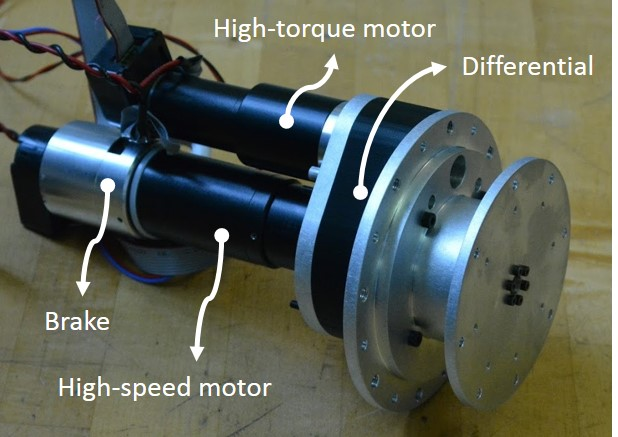
\includegraphics[width=0.60\textwidth]{dsdm_proto_2.jpg}
	\caption{DSDM actuator prototype}
	\label{fig:dsdm_proto}
\end{figure}

This technology allows for improved power transmission over a wide range of output speed, and reflecting radically different impedance at the output. Unlike alternative variable transmission approaches, this is achieved without requiring development of novel components, only proven technology (motor, brake and gears), which can be greatly advantageous from a product development point-of-view. 

\section{Motivation}
\label{sec:mot}

In many robotic systems, actuators are often required to operate in distinctively different torque-speed load conditions. A legged robot, for example, has to move its leg forward quickly through the air and, once touching the ground, it has to bear a large load \cite{hirose_study_1984}. These two operating conditions, high speed at low torque vs. high torque at low speed, are often an order of magnitude different, while the required output power is similarly low. When the torque-speed load conditions do not vary significantly, a single gear ratio can be picked so that the actuator always operate under nearly optimal conditions. For distinctively different torque-speed conditions, the actuator will be far for its optimal operating conditions with a gear ratio picked from the middle ground. As illustrated on Fig. \ref{fig:speedissue} for a typical electromagnetic (EM) actuator, extremum torque-speed conditions are not optimal in term of efficiency and power output. This often leads to the use of oversized and inefficient actuators, which is inhibitory particularly for mobile robots.

\begin{figure}[htp]
	\centering
		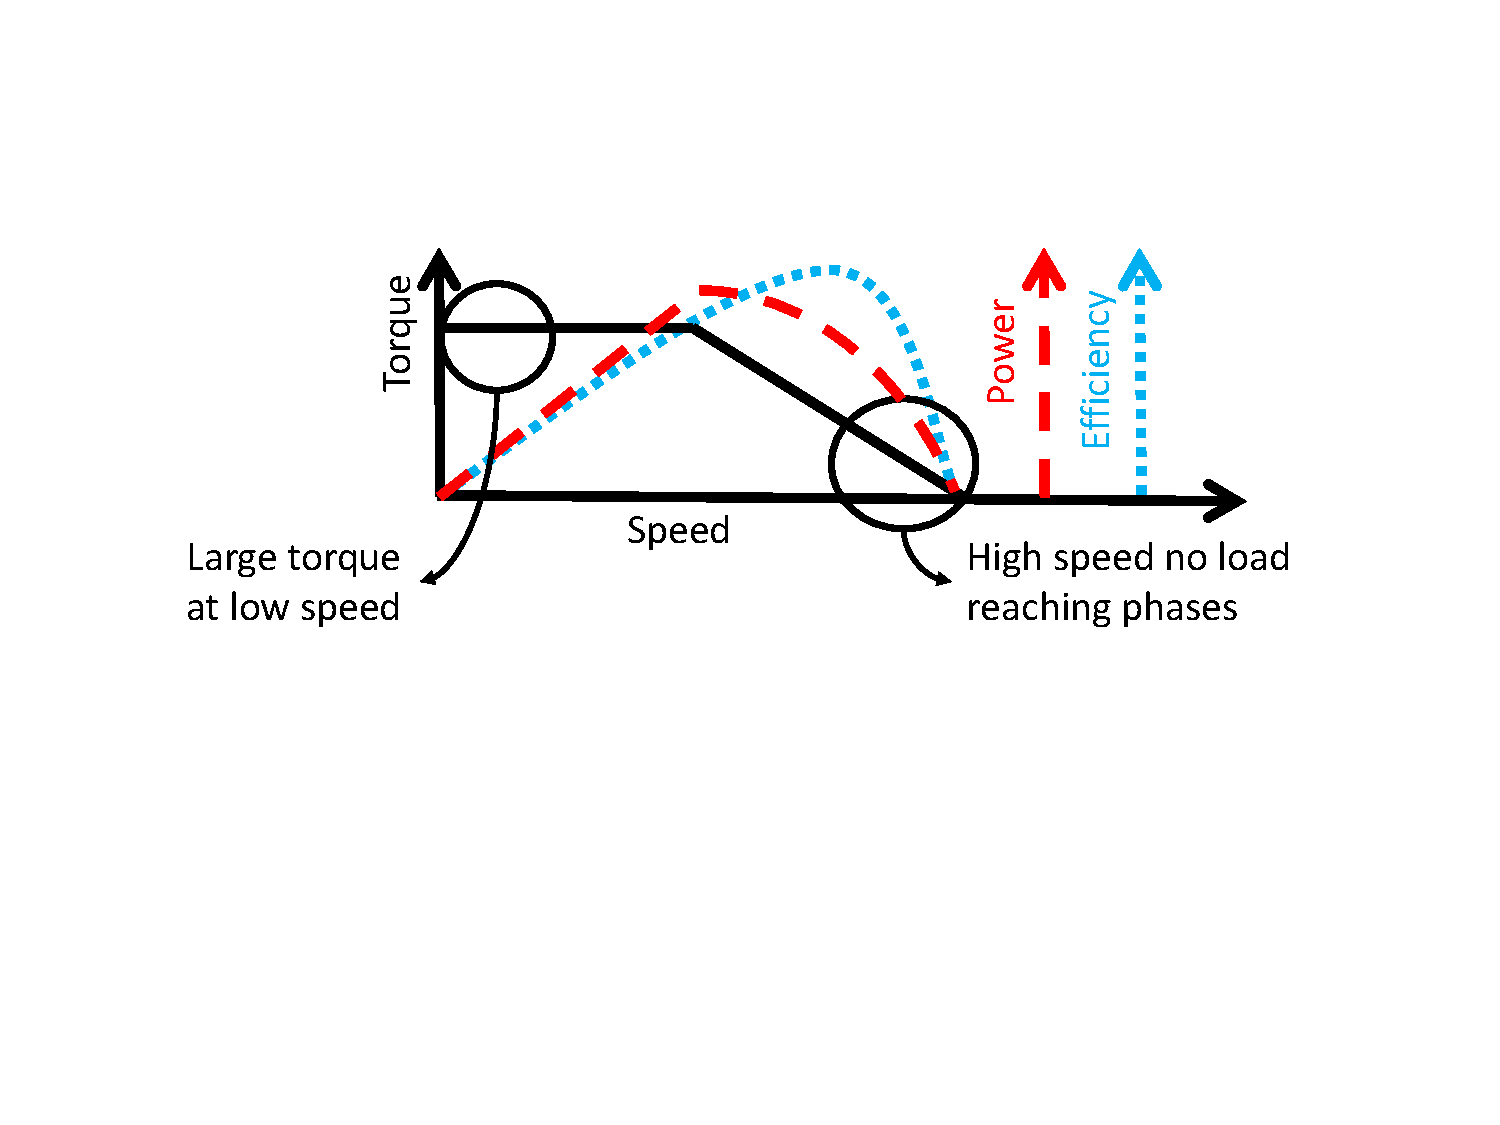
\includegraphics[width=0.70\textwidth]{speedissue.pdf}
	\caption{Limitations of EM motors for extremum torque-speed operations}
	\label{fig:speedissue}
\end{figure}

%EM motors cannot output high power at low speed because of thermal dissipation and magnetic flux limits related to material properties; are limited in speed by the supply tension and others; and are very inefficient when producing large forces at low speed \cite{hollerbach_comparative_1992}. 

Automobiles with internal combustion (IC) engines use transmissions with multiple gear-ratios to match torque-speed conditions. IC engines have a very narrow speed range in which they can effectively deliver power; a transmission with multiple gear ratios is a necessity for the engine to work effectively for a wide range of output speed. EM motors are more flexible than IC engines, but still far from ideal sources. EM motors cannot output high power at low speed because of thermal dissipation and magnetic flux limits related to material properties; are limited in speed by the supply tension and others; and are very inefficient when producing large forces at low speed \cite{hollerbach_comparative_1992}. In robotic, since it is often the extremums, i.e. maximum torque and speed, that determine the actuator design instead of the power requirement, much can be gained with multiple gear ratios.

It will be a significant breakthrough if a type of multiple speed transmission can be used effectively in robotics. Even a small, lightweight actuator can generate large torques and move at high speed if equipped with both large and small gear ratio. Moreover, a multiple gear-ratio transmission can allow an actuator to work closer to its optimal operating conditions, improving overall efficiency significantly. Furthermore, gear shifting significantly changes the intrinsic impedance of an actuator, since the impedance is proportional to the square of the gear-ratio. The actuator may be made back-drivable while using its small reduction ratio, an important property in many applications where the robot physically interacts with the environment \cite{hogan_impedance_2004}. Also the same actuator may be made non-back-drivable while using its large reduction ratio, allowing the actuator to support loads without consuming energy and enabling high-stiffness position control.



\section{Actuator and Powertrain Research}
\label{sec:actres}

\paragraph{Classical Actuators} Traditional robots generally use actuators that behave as displacement-sources because of their high intrinsic impedance. These include geared EM motors and hydraulics cylinders. Using a force sensor, it is possible to control the output force with this type of actuators, but the bandwidth is rather limited. To guarantee the stability of the force-feedback scheme only half the intrinsic inertia can be canceled \cite{hogan_impedance_2004}. Since 70's, roboticists have been attempting to build actuators that can behave naturally as a force-source such as series-elastic actuators, pneumatic cylinder and air-muscles \cite{hanafusa_stable_1977}\cite{pratt_series_1995}. However, because of the physical limitation of compliant transmission materials, the achievable bandwidth is limited and precise position control is hardly achievable. Direct drive EM actuators are the best force-source actuators with high fidelity, high bandwidth, and have been used for high-speed robots \cite{asada_direct-drive_1987} and more recently small legged robots \cite{kenneally_design_2016}. However, the very low force density \cite{hollerbach_comparative_1992} and low efficiency at low speeds make them impractical for most mobile robot applications, just holding a payload with static torques require continuous currents in the motors leading to a large energy consumption even though no mechanical work is done. 

Regarding power-throughput, as briefly discussed before and illustrated at Fig. \ref{fig:emcurve}, electromagnetic actuators are typically characterized by a flat force curve for most of their range of speed, leading to maximum power been only available at high velocity \cite{girard_two-speed_2015}. Fluidic actuator are typically characterized by a force curves droping quadratically with velocity (related to pressure losses in valves orifices), as illustrated at Fig. \ref{fig:fluidcurve}. All in all, EM and fluidic actuators are not perfect power sources and could benefit from using variable transmissions to have their maximum power available on a much wider range of speed.

\begin{figure}[htb]
        \centering
				\subfloat[Electromagnetic transducer]{
				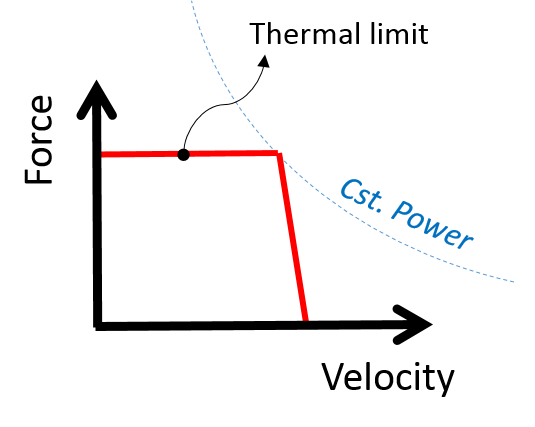
\includegraphics[width=0.35\textwidth]{EM_curve.png}
				\label{fig:emcurve}
				}
        \subfloat[Fluidic transducer]{
				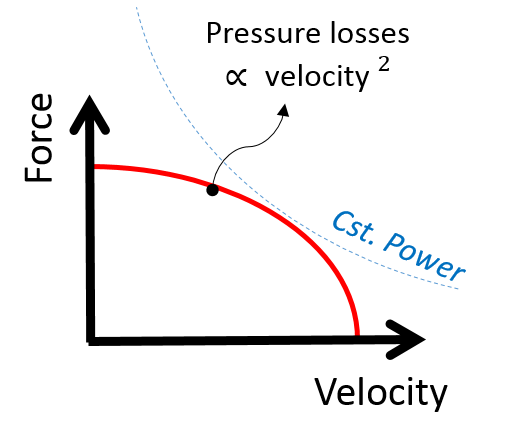
\includegraphics[width=0.35\textwidth]{fluid_curve.png}
				\label{fig:fluidcurve}
				}
        \caption{Typical force-speed curve of actuators}\label{fig:powercurves}
\end{figure}

Some advance electric motor systems can extend their operation at high-speed by weakening the magnetic flux. Such motors can thus transmit their maximum power over a wider range of speed than basic DC motors, see Fig. \ref{fig:EM_fluxweakening}. However, this clever electromagnetic scheme cannot go around the fundamental force saturation at low-speed, which is limited by material properties \cite{hollerbach_comparative_1992}. Hence, there is still a big advantage of using multiple gear-ratio even for motor using advance flux control schemes, see Fig. \ref{fig:EM_two}. 

\begin{figure}[htp]
	\centering
		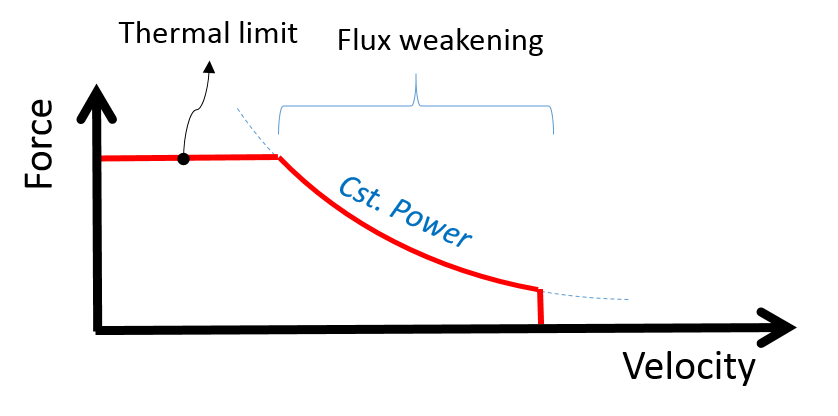
\includegraphics[width=0.5\textwidth]{EM_fluxweakening.png}
	\caption{Force-speed curve of electric motor using flux weakening }
	\label{fig:EM_fluxweakening}
\end{figure}

\begin{figure}[htp]
	\centering
		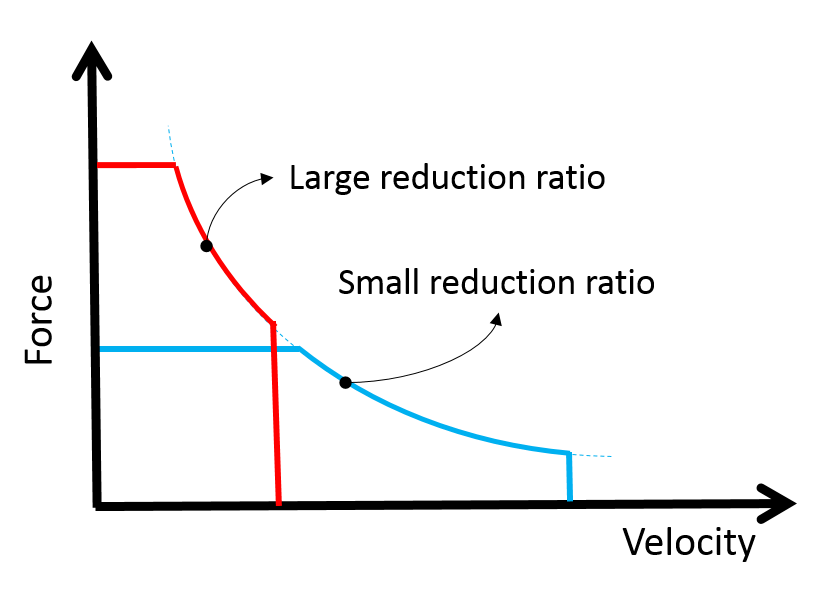
\includegraphics[width=0.5\textwidth]{EM_two.png}
	\caption{Force-speed curve of an electric motor using flux weakening with two different reduction ratio}
	\label{fig:EM_two}
\end{figure}


\paragraph{Variable Impedance Actuators} Force-source type of actuator are desirable for interaction tasks, for instance grasping, manipulation and locomotion, since the interaction force can be controlled. On the other hand, actuators with non-back-drivable mechanisms have the advantage for pure position controlled tasks, disturbance rejection and statically bearing large load without any power consumption. Since both small and large intrinsic impedances are advantageous in different scenario, several group have developed variable intrinsic impedance actuators, such as based on variable stiffness spring \cite{tonietti_design_2005}, antagonist non-linear devices \cite{koganezawa_antagonistic_2006}, a series-compliance that can be locked with a brake \cite{leach_linear_2012} and dual-motors in serial configuration \cite{kim_serial-type_2010}. Furthermore, so-called macro-micro actuators, can improve the bandwidth of force-source type of actuators by exploiting the high-bandwidth of a small actuator in parallel, allowing for wider-range impedance control and improved position control \cite{morrell_parallel-coupled_1998}. Regarding power throughput however, all these technologies are still limited by force-speed characteristic of their main transducer (generally a geared electric motor). Hence, those designs do not solve the problem of efficient power transmission over a wide range of speed.

\paragraph{Vehicle Powertrains} While the actuator work in robotics have been focused on impedance and bandwidth issues, in the powertrain field the torque-speed matching issue is predominant, since power density and efficiency are critical for mobile systems. The idea of using multiple gear ratios with electric motors has been explored occasionally, to improve efficiency and power density \cite{mckeegan_antonovs_2011}. A twin motor configuration has been proposed for smooth gear shifting, where each motor shifts at a different timing \cite{bologna_electric_2014}. Also, a dual motor configuration using a planetary coupling and non-back-drivable worm-gears was proposed for a mobile robot powertrain \cite{lee_new_2012}. Multiple gear-ratio powertrains provide effective solutions for torque-speed matching, but are not adapted to the robotic context. First because powertrain shift mecanism are not adapted to make gear shifts while interacting with dynamic environments, and second because they are designed to make shift between ratio much closer to one another than what is investigated in this thesis.

Fig. \ref{fig:forcefidelity} shows typical transmitted force profile during gear-shifts with powertrain shifting mechanisms. The simplest manual transmissions using dog clutch do not transmit torque at all during a shift, while more advance systems such as dual-clutch transmission can supply torque during the transition, the fidelity is low compared to what is typically expected from an actuator in a robotic context. For instance, with a state-of-the-art two-speed dual-clutch transmission for an electric car \cite{walker_powertrain_2017}, experimental results shows output torque oscillations with amplitudes of about 100\% the nominal value during a period of 500 ms. However, this torque deviation only lead to an undesirable car acceleration of about 0.05 g, and the effect is barely noticeable on the output velocity curve. As illustrated at Fig. \ref{fig:typeloads}, force fidelity requirement for vehicle powertrain are not very severe since the load is always a very large vehicle inertia which will act as a very strong low-pass filter. However, robotic system can be interacting with all kind of load without filtering characteristics. For instance, for a robot fighting a gravitational load or compressing a spring, it would be catastrophic if the force drop during a gear-shift. The output needs to be always fully under control in those situations. 

\begin{figure}[htp]
	\centering
		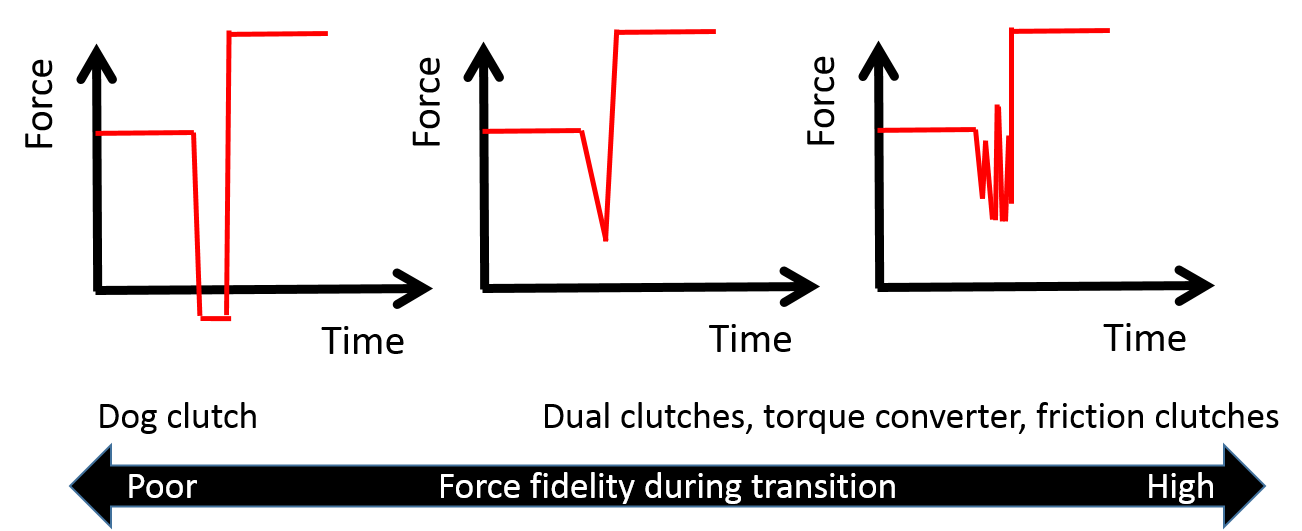
\includegraphics[width=0.90\textwidth]{forcefidelity.png}
	\caption{Force profile during a gear-shift with powertrain gear-shifting mecanisms}
	\label{fig:forcefidelity}
\end{figure}

\begin{figure}[htp]
	\centering
		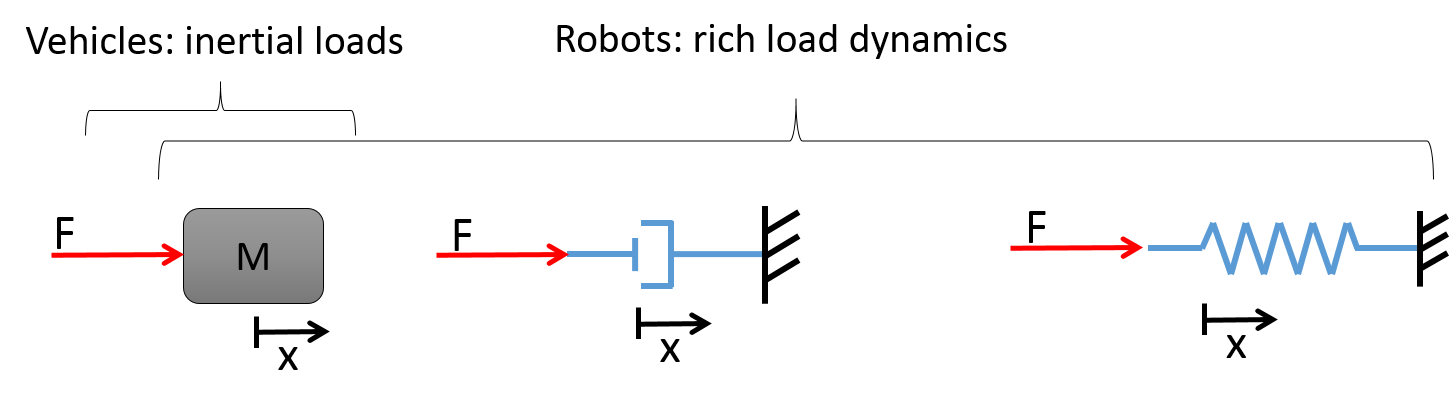
\includegraphics[width=0.90\textwidth]{typeloads.png}
	\caption{Type of loads encountered by vehicle powertrain vs. robot actuators}
	\label{fig:typeloads}
\end{figure}

One other aspect is that power-train gear-shifting mechanism are not adapted to make transition between drastically different gear-ratios. For instance, for dual-clutch system the ratio step between adjacent gear ratios should not exceed 1.8 to avoid shift difficulties \cite{gao_gear_2015}. Furthermore, from a design perspective, advance power-train systems are very complex machines (wet clutches, dry clutches, synchronizers, etc) leading to manufacturing, maintenance, wear and reliability challenges. Adding such systems in all the many actuators of a robotic system might be especially hard to justify when balancing all those practical issues. All-in-all, power-train gear-shifting technologies are not adapted directly for use in a general purpose robotic actuator.

%Continuously variable transmission (CVT) also are limited in term of total variation range, the variation from maximum to minimum ratio for those system are in the range of a factor of 3. 

\paragraph{Variable Gear-ratio Actuators} 
While variable gear-ratio actuators (VGA) have been studied extensively for automobile power-trains, they have not yet been fully investigated in robotics, despite significant potential gains. A few instance of research in that direction were made for legged locomotion \cite{hirose_design_1991}, grasping robotic hands \cite{shin_robot_2012} and actuators \cite{hirose_development_1999} \cite{byeong-sang_kim_improved_2007}\cite{tahara_high-backdrivable_2011}. While those works are promising, no gear shifting methodology for generic robot actuator in arbitrary dynamic situation are proposed.


\paragraph{Continuously variable transmissions (CVT)} 

Continuously variable transmission have been used sporadically for car power-trains. Most common design are based on belts with variable-diameter pulley or toroidal disk. Drawbacks compared to regular transmission include higher transmission losses and complex dynamics \cite{srivastava_review_2009}. Moreover, typical CVT total ratio variation are limited to a factor 4x (for instance 0.5:1 to 2:1), which makes them unadapted for very large ratio variation [TODO find a good CVT review article]. Some designs have been proposed for infinite range variation, often called IVT. For instance the company Torotrack claim to have a CVT that can reach an effective gear-ratio of zero \cite{schoolcraft_gear_2011}. However, since those designs rely on friction, maximum transmitted torque is limited and the transmission systems are complex and very large, which inhibit the potential use in robotic applications.

In the actuator field, lever mechanisms with variable attachment points that leads to a very wide range of effective transmission ratio \cite{tahara_high-backdrivable_2011}, even infinite range when using a singular configurations \cite{jafari_new_2014}, have been proposed. However, this type of CVT implementation limits drastically the motion range, thus cannot be used for general purpose actuator transmission. In the literature, those mechanisms are used in VSA between the spring and the output, where their limited motion range is not an issue. 

Many clever mechanisms have proposed to be used as CVT. However, all design have some major drawback regarding either: total variation range, constraints on output motion, ratio-variation speed, allowable shift conditions, efficiency, etc. The best indication of this is the automotive industry. On paper, there is a huge incentive to use CVT with internal combustion engine in because of their narrow peak of power and efficiency. However, despite a century of development in one of the largest industry, transmissions using many discrete gear-ratio are still the most widely adopted solution. Even with the recent effort to improve fuel economy, the trend in the industry is to use automatic transmissions with a large number of discrete gear \cite{phillips_10-speed_2010}\cite{goleski_multi-speed_2015}. Furthermore, compared to the automotive field, the incentive of using CVT in robotics is diminished because of more flexible torque curves of electric motor and the wider desired range of ratios. Hence, all the limitations of CVT make this technology unadapted for general purpose robotic actuators. However, a breakthrough in term of IVT technology would be very interesting for the field of robotics.

\subsection{Novel Contribution}
%\paragraph{Novel Contribution} 
The presented DSDM actuator in this chapter, address the issue of improving available power and efficiency over a wide range of operating speeds, which has rarely been addressed in the robotics literature. Also, the actuator enable order-of-magnitude variation of the output impedance, which is also a highly desirable feature.  \textbf{The main novel contribution is the methodology for gear shifting between two very different gear-ratios seamlessly even in highly dynamic situations, which is a key enabling feature for robotic applications.} A mechanical architecture where two motors are coupled using a 3-ports gearbox and a brake is used in conjunction with novel control scheme to provide full control of the output during gear shifting. The mechanical architecture is not new by itself as similar architectures (using planetary and brakes) are used in hybrid car powertrains, automatic transmissions and special actuators. However, here this architecture is used in conjunction with a novel controller to provide full control of the output during gear shifting. A preliminary version of this work have been published in \cite{girard_two-speed_2015}, but this chapter include a more throughout analysis and new algorithms for fast gear-shift even during impacts. 

To the knowledge of the author, no other technology can meet all those requirements:
\begin{itemize}
	\item Fast shifting between order-of-magnitude different gear-ratios
	\item High-fidelity control of the output during transitions
	\item Simple mechanical design enabling small and practical implementations
\end{itemize}

\subsection{Related works}
%\paragraph{Other dual-motor actuators} 
Many dual-motor actuators have been proposed in the literature \cite{tagliamonte_double_2012}, with different goals and architectures. So called macro-micro actuators, see Fig. \ref{fig:macromicro}, are essentially series-elastic actuators equipped with an additional small motor directly attached to the output. Variable stiffness actuators (VSA), see Fig. \ref{fig:vsa}, are also series elastic actuators where a small motor can modulate either the spring directly or the transmission between the spring and the output.
%
\begin{figure}[htp]
        \centering
				\subfloat[Macro-Micro \cite{morrell_parallel-coupled_1998}]{
        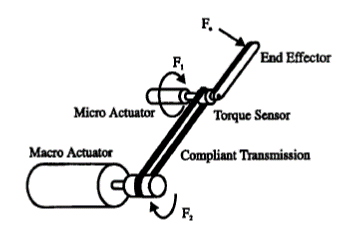
\includegraphics[width=0.45\textwidth]{macromicro.png}
				\label{fig:macromicro}}
        \subfloat[Variable stiffness \cite{jafari_new_2014}]{
				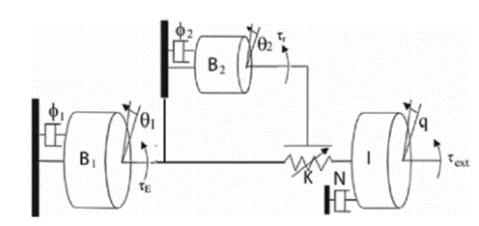
\includegraphics[width=0.45\textwidth]{VSA.png}
				\label{fig:vsa}}
        \caption{Dual-motor architectures}\label{fig:dualmotoractuators}
\end{figure}
%
Fig. \ref{fig:variableimpedanceactuators} shows a generalized bond-graph actuator model illustrating the conceptual differences between many approaches. Variable stiffness actuators use a variable transmission placed between a compliant element and the load, where it influence the reflected output stiffness but not the steady-state power-transmission characteristics. Macro-micro actuators have a fixed reflected output stiffness, but the advantage is that the additional direct-drive motor on the output makes possible to emulate a wide-range of output impedance. \textbf{The proposed VGA actuators in this thesis are fundamentally different, it is the transmission between the motor and the load that is varied, like in a car transmission.} The main advantage of VGA is regarding efficient power transmission, enabling small motors to make full use of their maximum power at high speed and at low speed. Macro-micro actuators and VSA have no advantages over a regular electric motor regarding the range of speed at which power can be transmitted. On the other hand, macro-micro and VSA have the ability to store and release potential energy in their compliant element, which is not the case with VGA. Regarding, natural reflected impedance, both VSA and VGA have the ability to change it. One fundamental difference is that VGA can only attenuate or amplify the natural inertia and friction of the rotor, while VSA can only modify its reflected stiffness. 

\begin{figure}[htp]
	\centering
		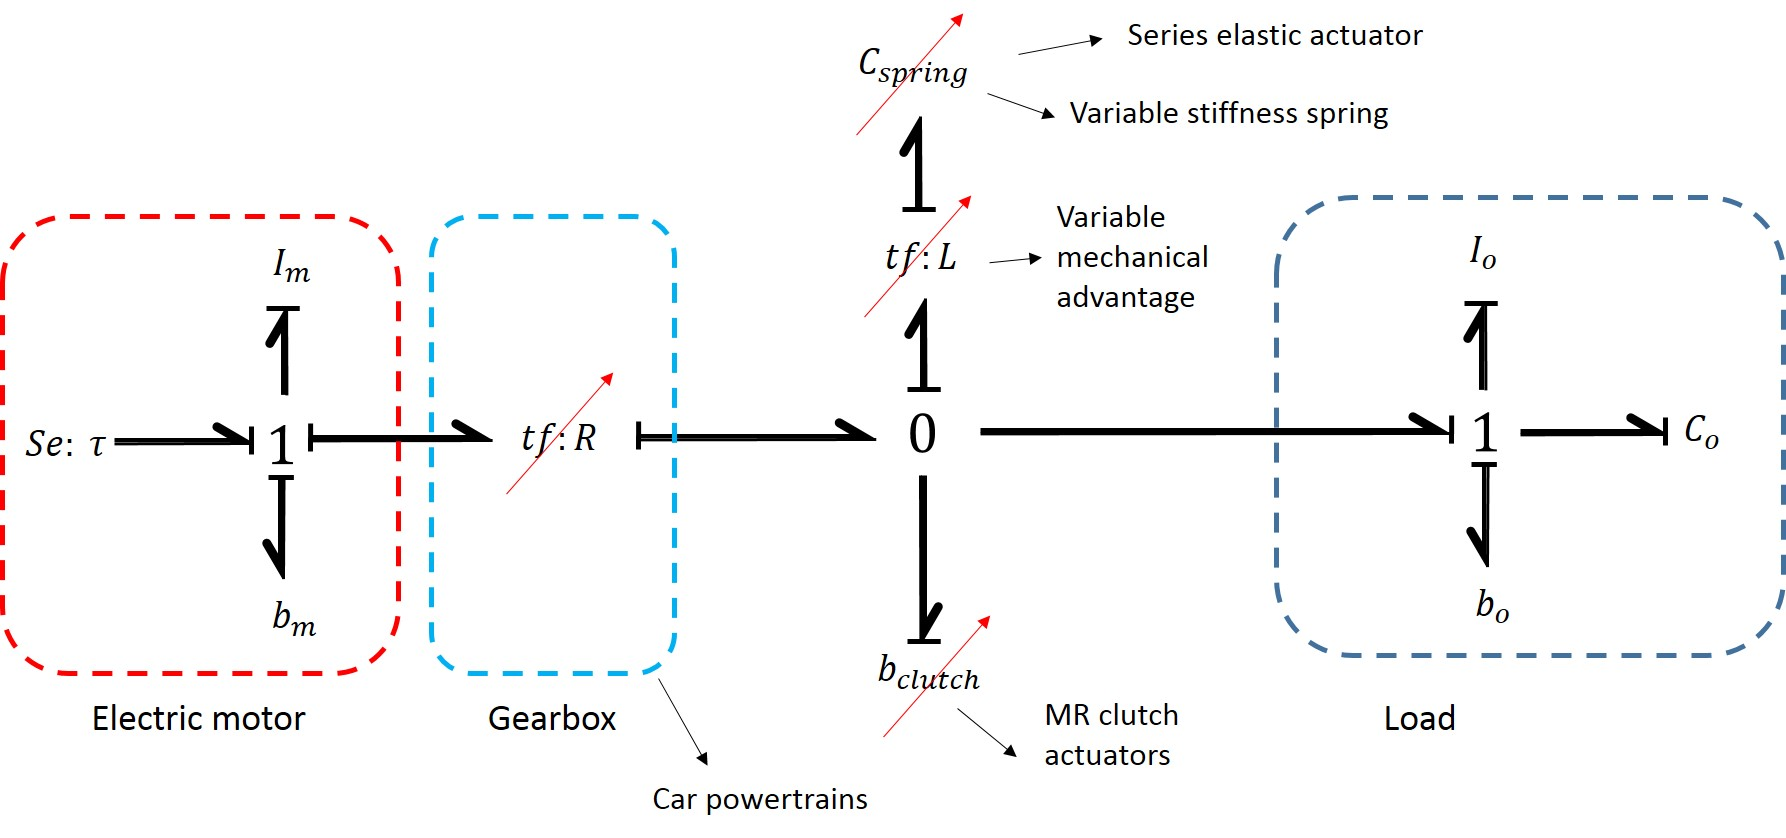
\includegraphics[width=0.90\textwidth]{variableimpedanceactuators.jpg}
	\caption{Different approaches for variable impedance actuators}
	\label{fig:variableimpedanceactuators}
\end{figure}




%%%%%%%%%%%%%%%%%%%%%%%%%%%%%%%%%%%%%%%%%%%%%%%%%%%%%%%%%%%%%%%%%%%%%%%%%%%%%%%%%%%%%%%%%%%%%%%%%%%%%%%%%%%%%%%%%%%%%%

\newpage

\section{Dual-Speed Dual-Motor architecture}
\label{sec:DSDM}

The proposed architecture, referred to as a Dual-Speed Dual-Motor (DSDM) actuator, consists of a direct drive motor (M1) equipped with a locking brake and an geared EM motor (M2) with a large reduction ratio coupled to the same output through a differential, see Fig. \ref{fig:dualmotorconcept}. The differential can be viewed as a 0-type junction (taking bond-graph terminology) where the speeds add up and the force is shared. 


\begin{figure}[H]
	\centering
		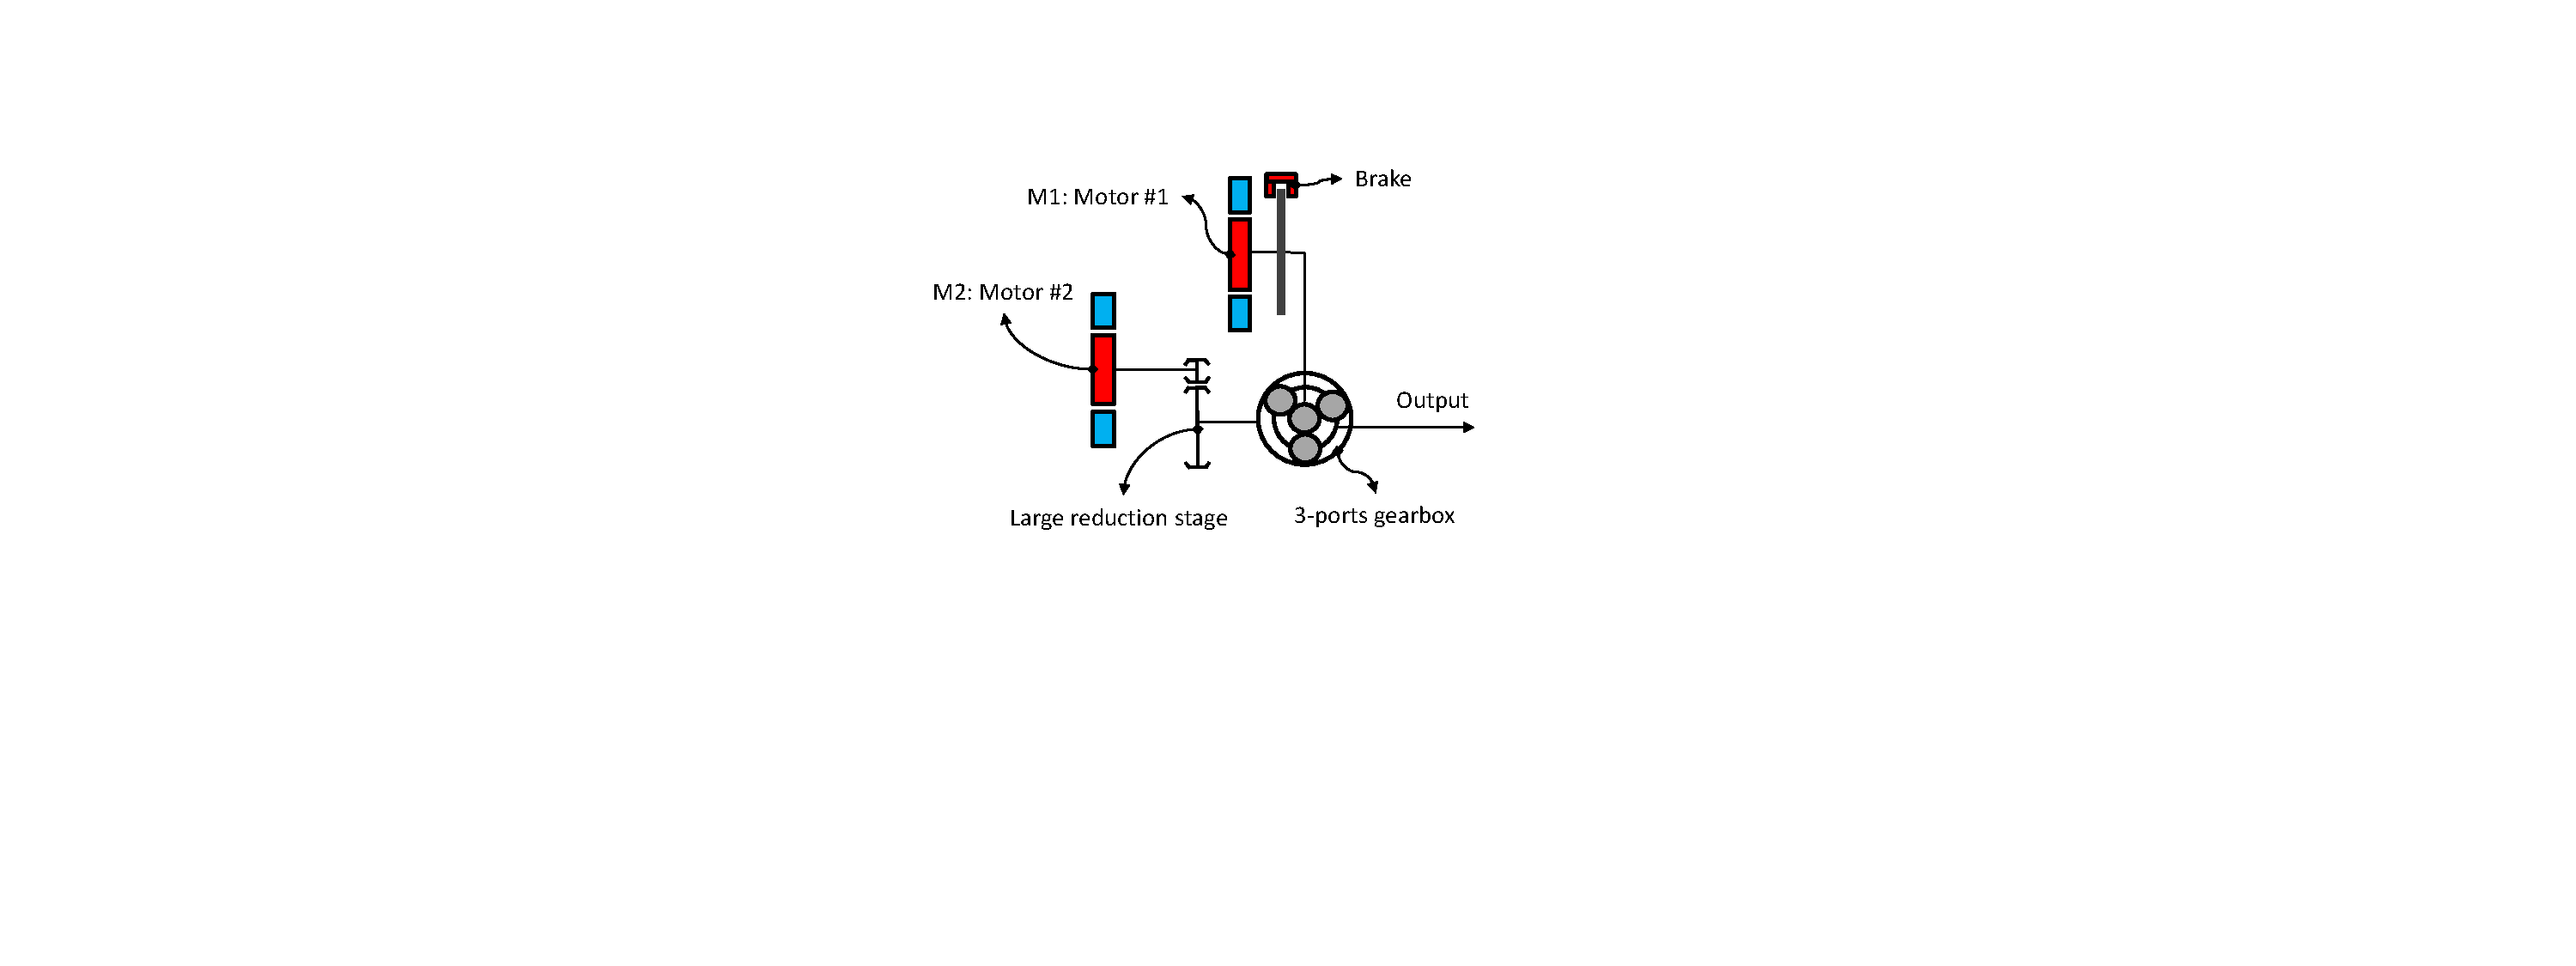
\includegraphics[width=0.60\textwidth]{dualmotorconcept2.pdf}
	\caption{DSDM actuator concept}
	\label{fig:dualmotorconcept}
\end{figure}

The envisioned implementation of the DSDM concept is to embed all the components into a single compact unit, as illustrated by Fig. \ref{fig:embedded}. A lot of weight and space could be saved by combining the reduction and the differential gearing and having all the components inside a single housing. 


\begin{figure}[H]
	\centering
		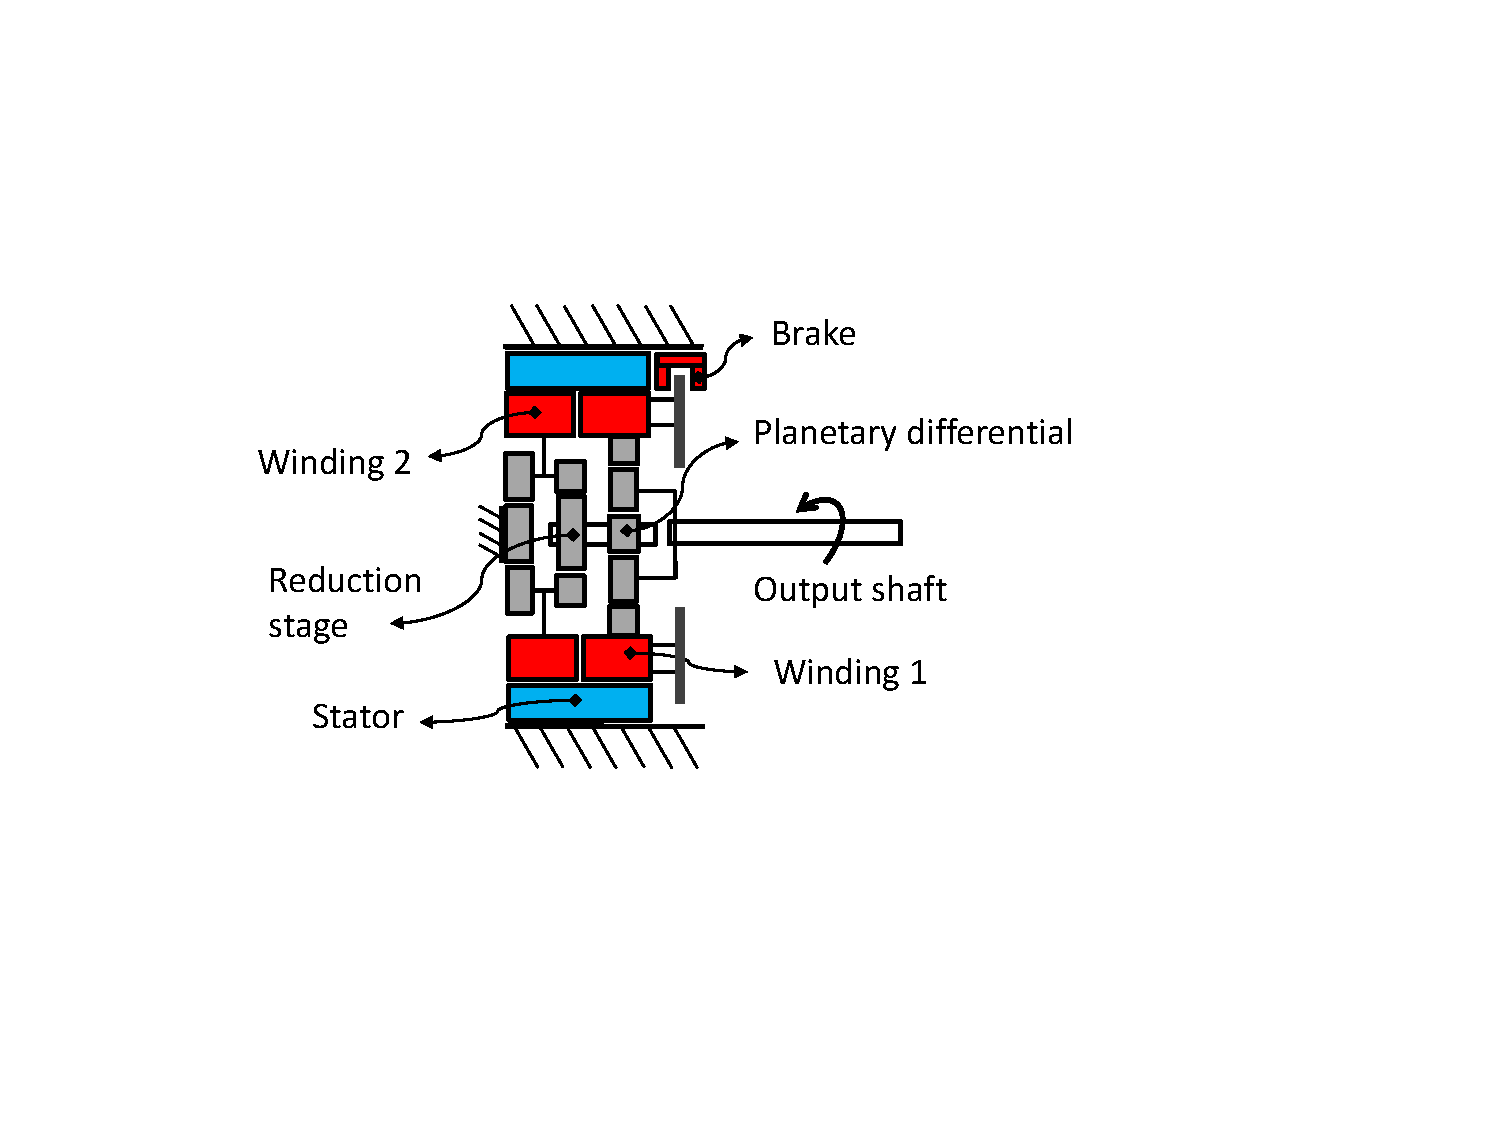
\includegraphics[width=0.60\textwidth]{embedded3.pdf}
	\caption{Possible architecture of an integrated DSDM concept}
	\label{fig:embedded}
\end{figure}

Fig. \ref{fig:embedded} shows a prototype of a DSDM actuator with a revolute output, using discrete off-the-shelf motors for modularity and ease of implementation.


\subsection{Principle}
\label{sec:princ}



The DSDM can be used in two modes, high-force mode when the brake is closed and high-speed mode when the brake is open. The result is like having two very different reduction ratio you can choose from during operation. Fig. \ref{fig:lever} conceptually illustrates the principle with a leverage analogy, M1 acts like a force source connected almost directly to the output and M2 acts like a displacement source with a large lever arm relative to the output. 
%
\begin{figure}[H]
	\centering
		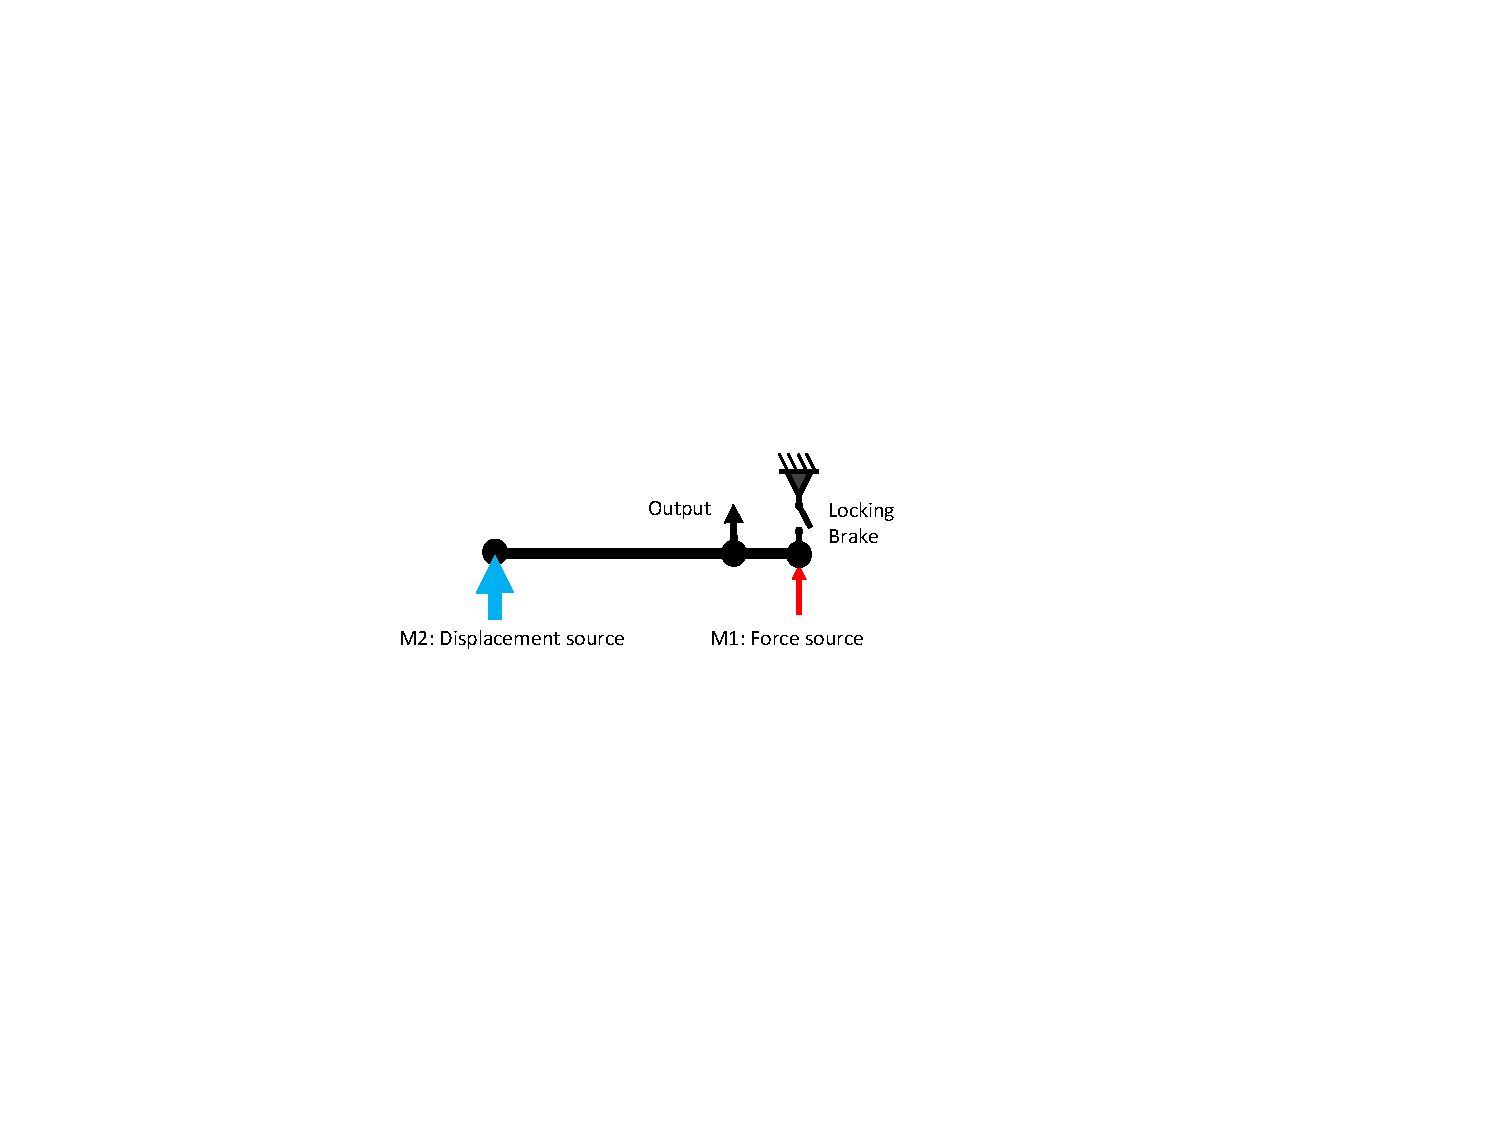
\includegraphics[width=0.60\textwidth]{lever.pdf}
	\caption{Dual input system}
	\label{fig:lever}
\end{figure}
%
During the high-force mode, see Fig. \ref{fig:HF}, the brake is closed and M2 drives the output with a large mechanical advantage. The result is a low-speed displacement-source type of actuation like a geared EM motor. During the high-speed mode, see Fig. \ref{fig:HS}, M1 drive the output almost directly, creating a high-speed force-source actuator like a direct drive EM motor. Additionally, both motors can be used simultaneously to drive the output even faster.
%
\begin{figure}[H]
        \centering
				\subfloat[High force mode (brake closed)]{
        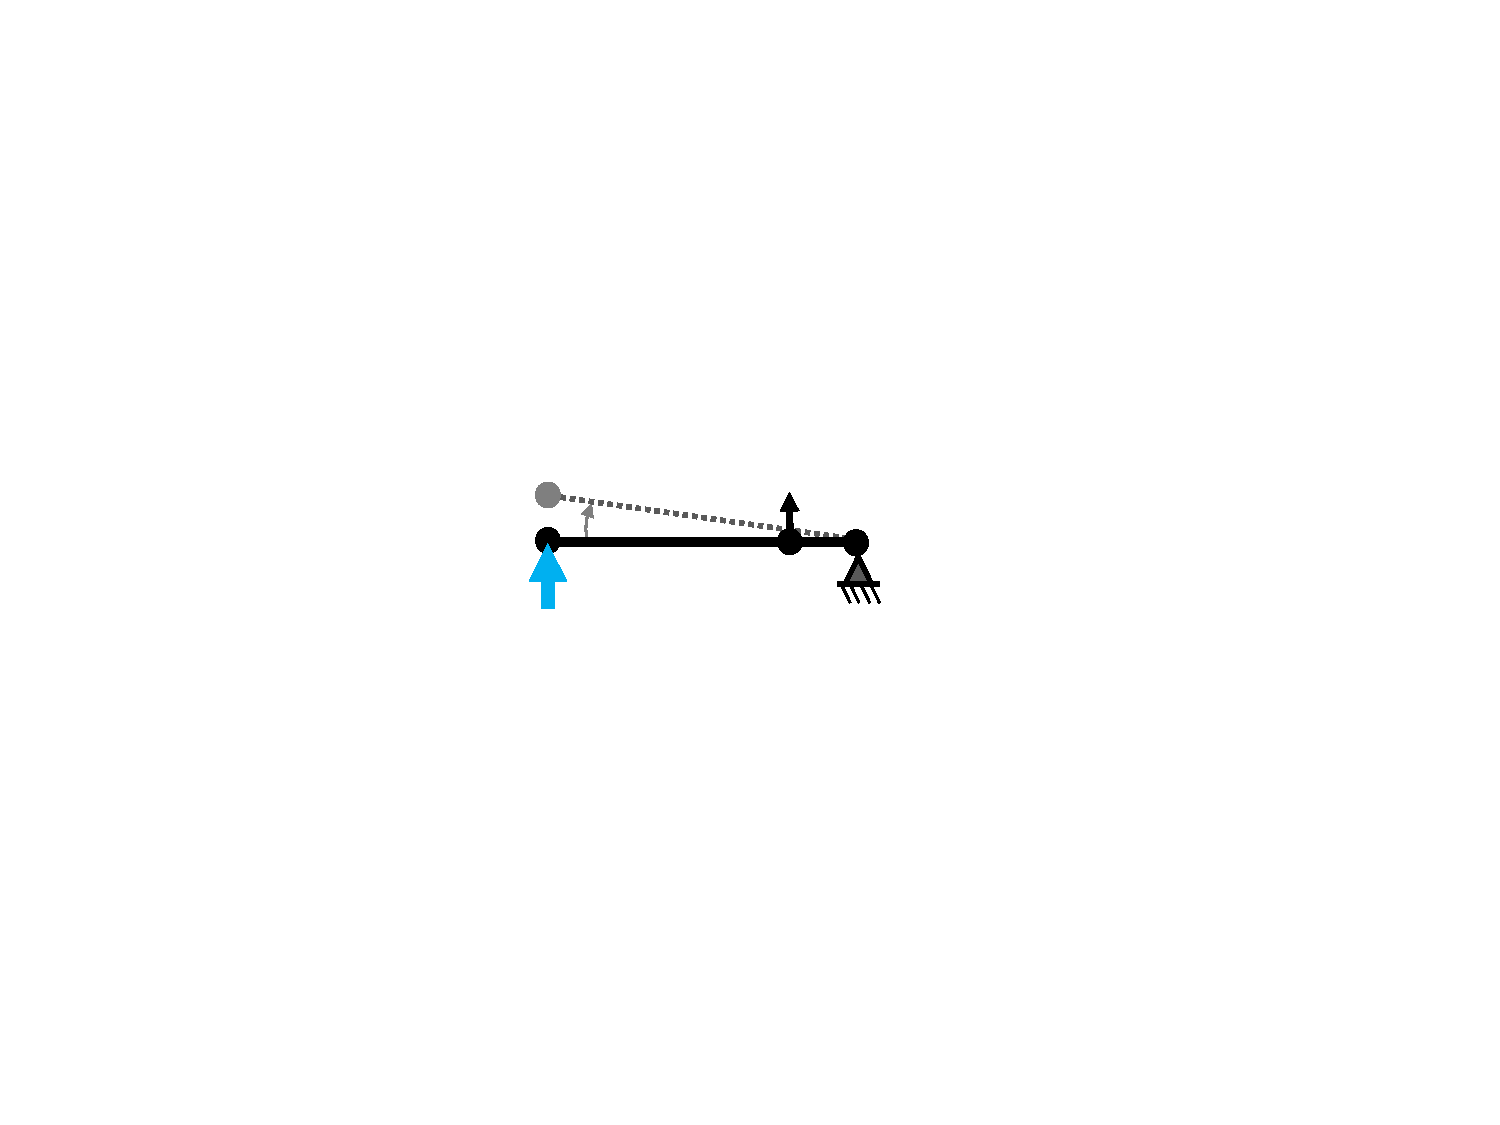
\includegraphics[width=0.38\textwidth]{leverHF.pdf}
				\label{fig:HF}}
        \subfloat[High speed mode (brake open)]{
				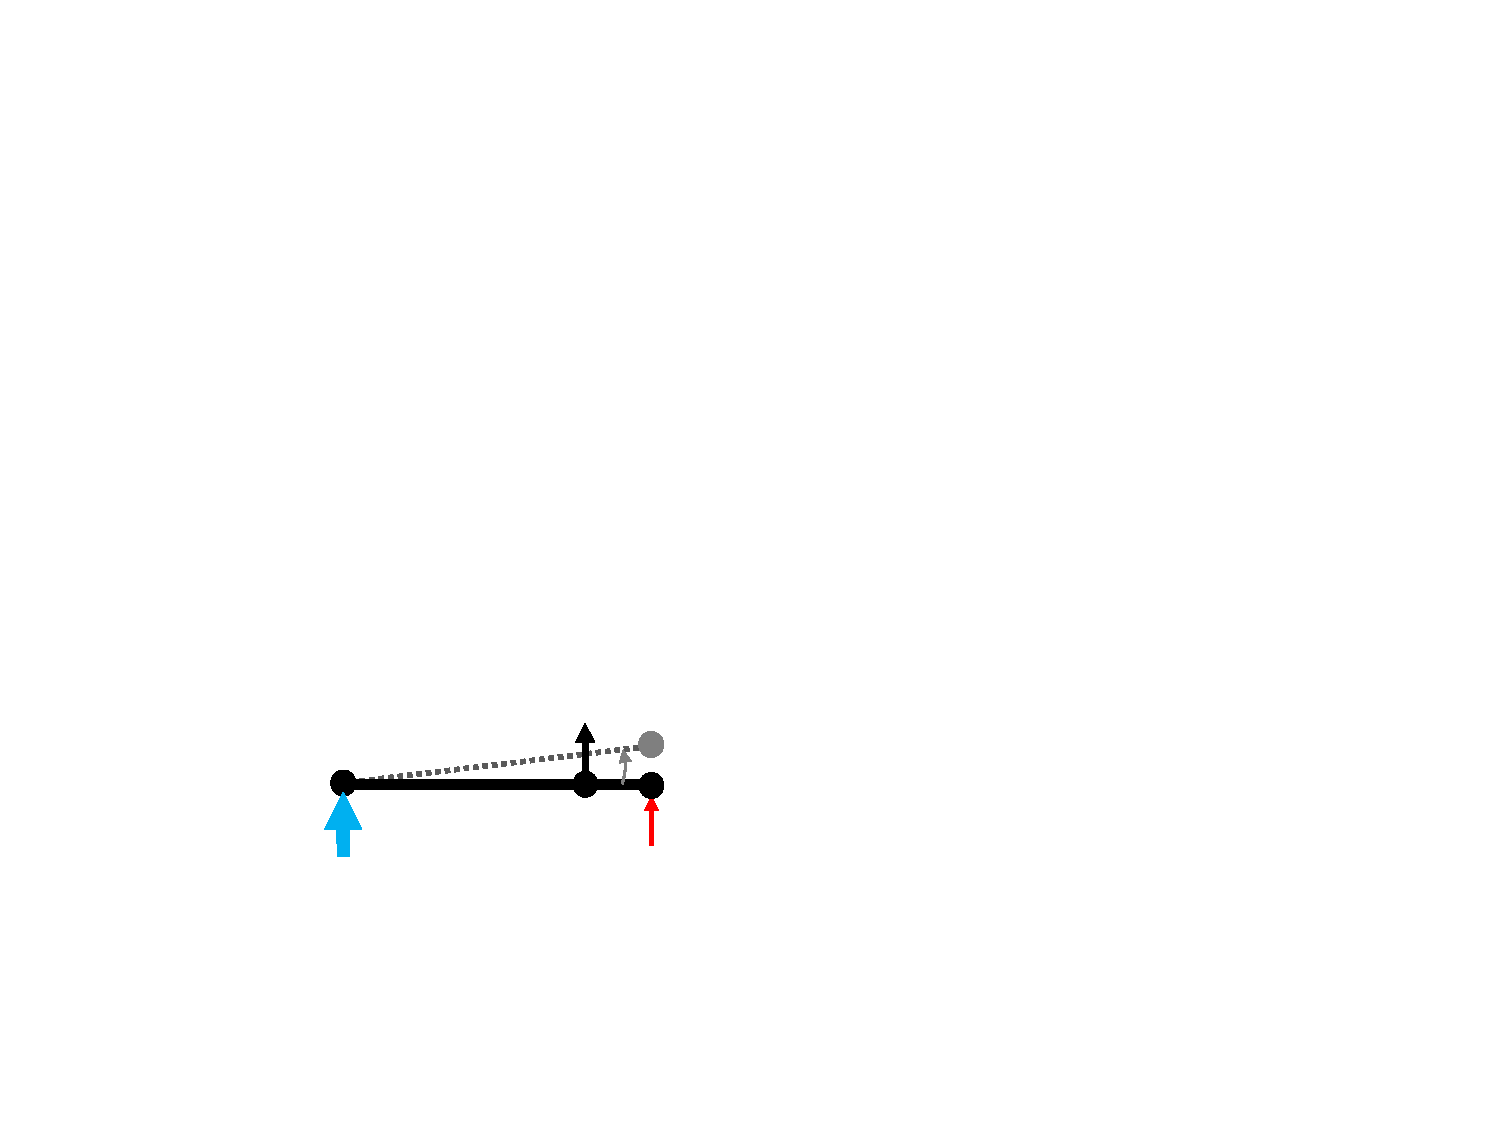
\includegraphics[width=0.38\textwidth]{leverHS.pdf}
				\label{fig:HS}}
        \caption{Two modes of operation}\label{fig:opmode}
\end{figure}

Fig. \ref{fig:torquespeed} illustrates the operating range of the DSDM actuator plotted on the standard torque-speed plane. The high-force mode region is determined by the performance of M2 alone, since M1 is locked. The high-speed mode region can exceed the performance of M1 alone, as M2 can be used simultaneously to increase the output speed. The fail safe zone indicate the guaranteed performance of the DSDM actuator in case of failure in either motor. 

\begin{figure}[H]
	\centering
		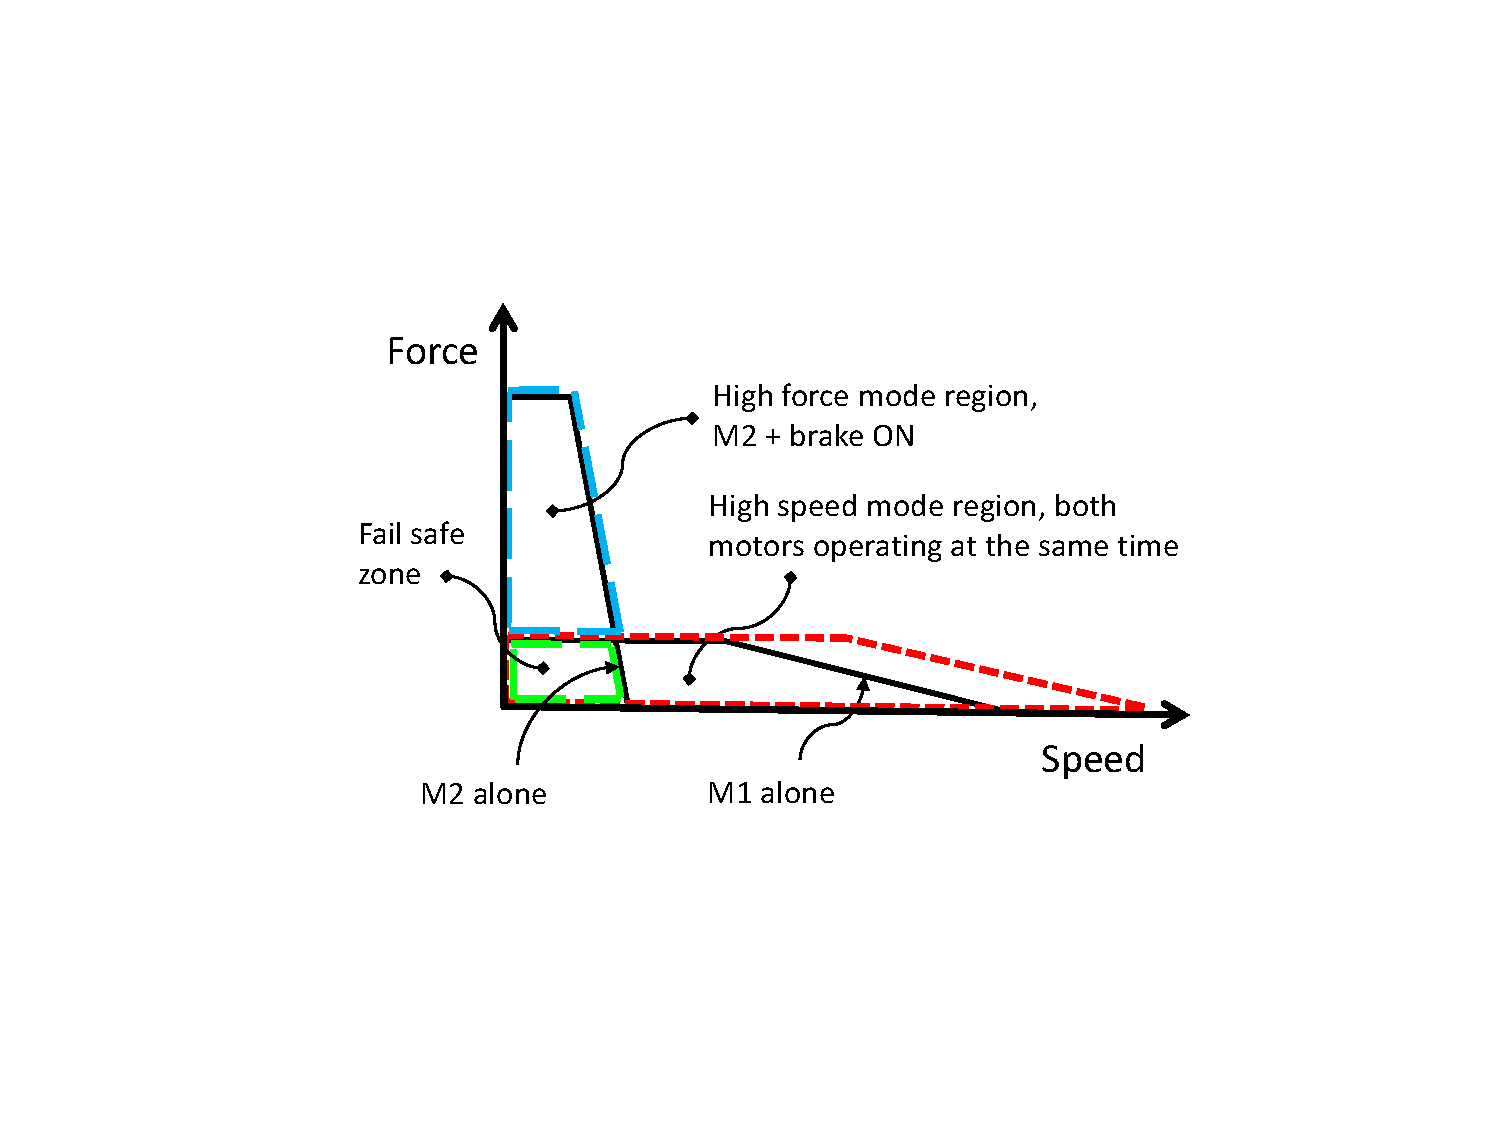
\includegraphics[width=0.65\textwidth]{torquespeed.pdf}
	\caption[DSDM actuator operation region]{DSDM actuator operation region, with a difference between M1 and M2 gearing ratio of only 4 for illustration purposes }
	\label{fig:torquespeed}
\end{figure}

\subsection{Weight advantage}
\label{sec:WeightAdvantage}


A DSDM actuator will be lighter than a single motor for applications with a wide range of operating speed. Suppose that an actuator must generate 10 W output power at two operating points: 0.5 Nm of torque at a speed of 20 rad/sec and 0.1 Nm at 100 rad/sec. A single EM motor that satisfies these requirements at both operating points tends to be oversized in terms of power, to reach both operating points, see Fig. \ref{fig:s1}. A DSDM actuator can reach the same operating points using two smaller motors with appropriate gear ratios, see Fig. \ref{fig:s2}. On the other hand the DSDM actuator uses more components: two motors instead of one, more gearing and an additional brake. The DSDM concept pays-off when the difference in speed between two required operating points becomes larger.  Fig. \ref{fig:1vs2} shows the estimated weight of actuators in relation to the ratio of operating speeds ($\lambda=\frac{w_1}{w_2}$), while the required power output is kept at 10 W. The actuator weight is computed assuming that the mass of each component is proportional to its maximum output torque, with values taken from commercially available components in the 10 - 100 watts range: 2 kg/Nm for motors, 0.1 kg/Nm for gearboxes and differentials and 0.2 kg/Nm for brakes \cite{maxon_motor_usa}. As shown in Fig. \ref{fig:1vs2}, the DSDM concept becomes advantageous when there is a large speed difference between the operating points. This is because only the gearbox and brake need to be scaled up for the DSDM actuator to meet the high torque requirement of the low-speed operating point, while the motor size must be increased for the single motor solution.

\begin{figure}[H]
        \centering
				\subfloat[One motor solution]{
				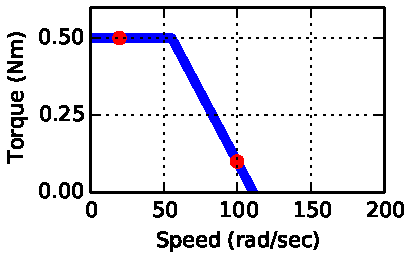
\includegraphics[width=0.42\textwidth]{sol1.pdf}
				\label{fig:s1}}
        \subfloat[DSDM solution]{
				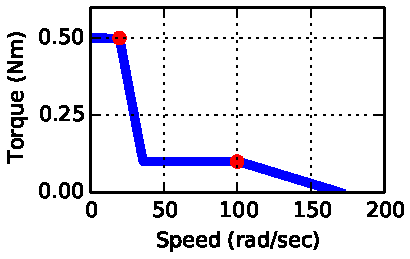
\includegraphics[width=0.42\textwidth]{sol2.pdf}
				\label{fig:s2}}
        \caption{Case study of two actuator solution for two 10 W operating points }\label{fig:solutions}
\end{figure}

\begin{figure}[H]
	\centering
		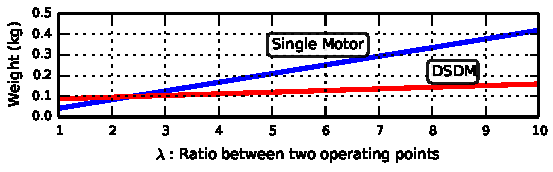
\includegraphics[width=0.75\textwidth]{w_vs_ratio.pdf}
	\caption[DSDM weight analysis]{Weight of a single motor compared to the DSDM concept for two 10 W operating points at different speeds $w_1=100$ rad/sec, $w_2 = w_1 / \lambda$}
	\label{fig:1vs2}
\end{figure}

Note that a two-speed actuator using a single motor and a variable transmission similar to the type used in car power-trains could have an even larger weight advantage over a single-gear motor. However, this type of variable transmissions, using components such as dog clutch, synchronizers and friction clutches, would not exhibit the features required to change gear-ratio seamlessly in the dynamic situations encountered by robots, unlike the DSDM architecture.

\subsection{Efficiency advantage}
\label{sec:EffAdvantage}

VGA actuators, including DSDM actuators, can transmit power more efficiently given various operating conditions. Electric motor efficiency is a function of velocity and applied torque. The efficiency map depends on the electric motor type (DC brushed, AC induction, DC brushless, etc). As a general rule, motors are typically more efficient in the upper-end of their velocity range. Hence, by using multiple gear-ratios, not only motors can be down-sized, but power transmission can be made more efficient. For instance, switching to a large gear-ratio to use a motor at its most efficient operating conditions. This efficiency advantage has been studied for electric cars equipped with multiple speed transmissions \cite{ren_effect_2009} \cite{holdstock_energy_2012} \cite{zhang_three-speed_2013} \cite{mckeegan_antonovs_2011}. This advantage is also of high interest for any mobile robot where on-board energy is limited. Any quantitative analysis of this benefit depends heavily on the specific of the type of motor used, the controller, the robotic system and the task executed by the robotic system. Section \ref{sec:shift_sim} will offer some quantivative simulation results regarding reduced energy consumption of robotic manipulator achieved using VGA actuators.

Another significant efficiency advantage of DSDM actuators over single-gear motors, is that high-speed mode can be backdrivable for interaction tasks while the high-force mode can be made non-backdrivable (using a irreversible large reduction for M2) in order to be able to hold an object against gravity without having to consume any electrical energy. A backdrivable single-gear motor will always have to supply electrical power just to sustain gravity forces, leading to zero efficiency for holding tasks. Hence, for a robot requiring backdrivability in some task and often holding objects against gravity, the efficiency gain could be huge. Note that some industrial robot arms use brake mounted on actuator outputs to address this type of energy consumption issue \cite{meike_energy_2011}.

An additional advantage of the DSDM architecture, is that during high-speed operation, many combination of M1 and M2 velocity can lead to the same output velocity. Hence, this internal degree of freedom can be used to further optimize efficiency by distributing motor speeds to minimize the overall energy consumption. 


\subsection{Reliability advantage}
\label{sec:RelAdvantage}

An additional secondary advantage of the DSDM architecture is that some minimum performance, illustrated by the green area at Fig. \ref{fig:torquespeed}, can be guaranteed even if either motor fail. Here failures leading to either jamming (rotor and stator stuck together) or freewheeling (motor cannot transmit any torque) are considered. 

\paragraph{Jamming of M1}
If M1 jams, then the situation is the same as if the brake would be engaged, and the capability of high-force mode is still available.

\paragraph{Jamming of M2}
If M2 jams, then M1 can still be used freely to move the output. The capability of high-speed are almost fully available, only the maximum speed is reduced as M2 is not available to add-up speed.

\paragraph{Freewheeling of M1}
If M1 is no longer able to transmit any torque, than if the brake is engaged all the capability of high-force mode are still available. 

\paragraph{Freewheeling of M2}
If M2 is no longer able to transmit any torque, M1 can still be used to move the output. Assuming the reduction stage of M2 is irreversible or barely backdrivable (meaning its associated moving part in the differential is still fixed and can sustain reaction forces) then the capability of high-speed are fully available.

%\section{Fast and Seamless Gearshifts}
%\label{sec:FastAndSeamlessGearshifts}

\newpage

\section{Modeling}
\label{sec:mod}

This section derives mathematical equations describing the behavior of a DSDM actuator for the purpose of designing adequate control laws. 

\subsection{3-ports Planetary Gear Junction}

\begin{figure}[htp]
	\centering
		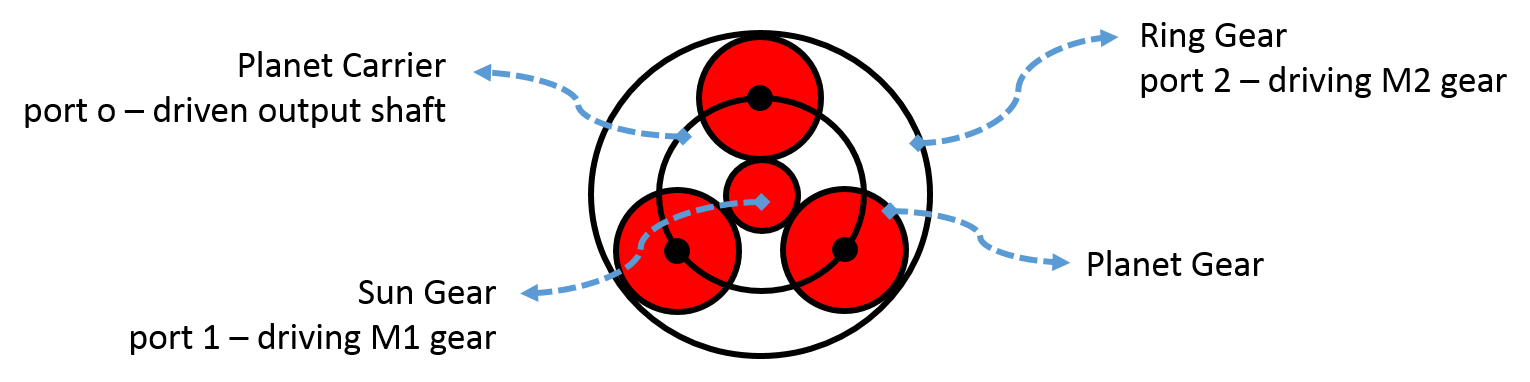
\includegraphics[width=0.85\textwidth]{planetary.png}
	\caption{Planetary gear-box used as a 3-port junction}
	\label{fig:planetary}
\end{figure}

A planetary gear box is used to implement the differential junction that links the two motors to the output. As illustrated by Fig. \ref{fig:planetary}, the planet carrier is connected to the output, M1 to the sun gear and M2 to the ring gear. Note that in typical gear-reducers using a planetary, the ring gear is usually fixed and there is a single DoF in the gearing. Here the ring gear is also mounted on bearing and there is 2 DoF in the gearing. The kinematic relation of the system is given by
%
\begin{align}
	w_o = 
	\underbrace{ \left[ 
	\frac{ 1 }{N+1}
	\right] }_{  1/R_1  }
	w_1 + 
	\underbrace{ \left[ 
	\frac{ N  }{r_2 (N+1)}
	\right] }_{  1/R_2  }
	w_2
\label{eq:kinematic}
\end{align}
%
where $r_2$ is the additional reduction of M2, $N$ is the ratio of gear teeth of the ring gear over the sun gear, and $w_o$, $w_1$ and $w_2$ are angular velocities of the output shaft (port $o$), M1 input shaft (port $1$) and M2 input shaft (port $2$). Neglecting internal inertial forces in the gearing, the effort relation of the system is given by:
%
\begin{align}
	- e_o =
	\underbrace{ \left[ 
	N+1
	\right] }_{ R_1  }
	e_1 = 
	\underbrace{ \left[ 
	\frac{r_2(N+1)}{N}
	\right] }_{ R_2  }
	e_2
	\label{eq:torque}
\end{align}
%
Hence, the 3-ports planetary coupling can be interpreted as a 0-junction, in the bond graph terminology, with different mechanical advantages ($R_1$ and $R_2$) on each input ports. 

\subsection{Dynamics}
\label{sec:dyn}

Fig. \ref{fig:dynamics} shows a lumped-parameter dynamic model of a DSDM when the brake is open (high-speed mode). $I_i$ and $b_i$ are the inertia and damping of the respective i-th ports. It will be assumed here that low-level high-bandwidth current controller are used, and electromagnetic torques $\tau_1$ and $\tau_2$ are going to be considered directly as inputs to the system. An equivalent bond-graph model is illustrated at Fig. \ref{fig:dynamics_bond}.

\begin{figure}[htb]
	\centering
		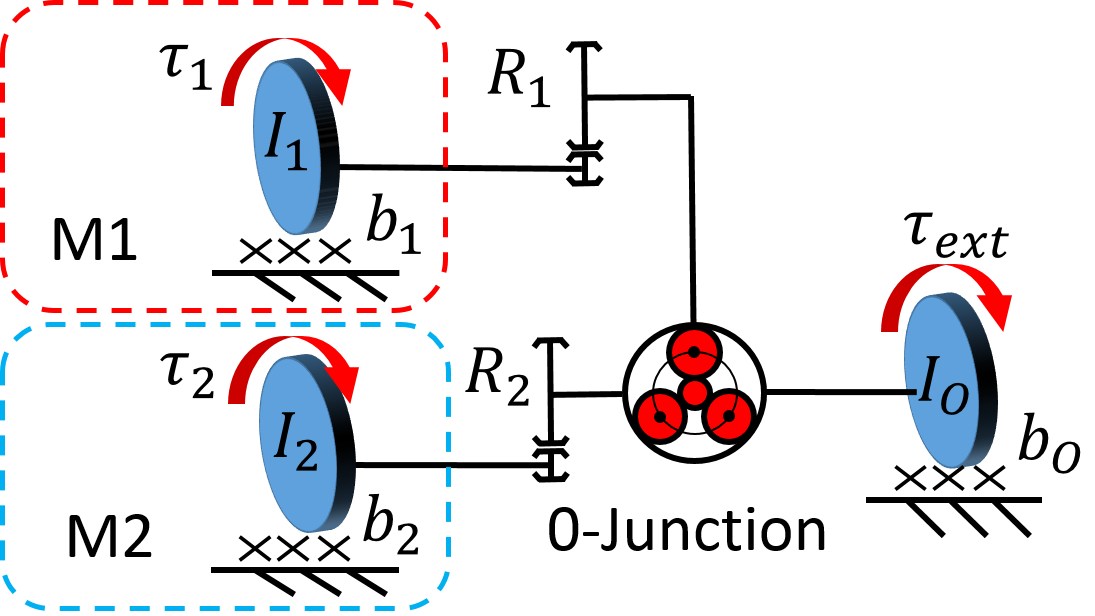
\includegraphics[width=0.65\textwidth]{dynamics.png}
	\caption{Lumped-parameter dynamic model of a DSDM}
	\label{fig:dynamics}
\end{figure}

\begin{figure}[htb]
	\centering
		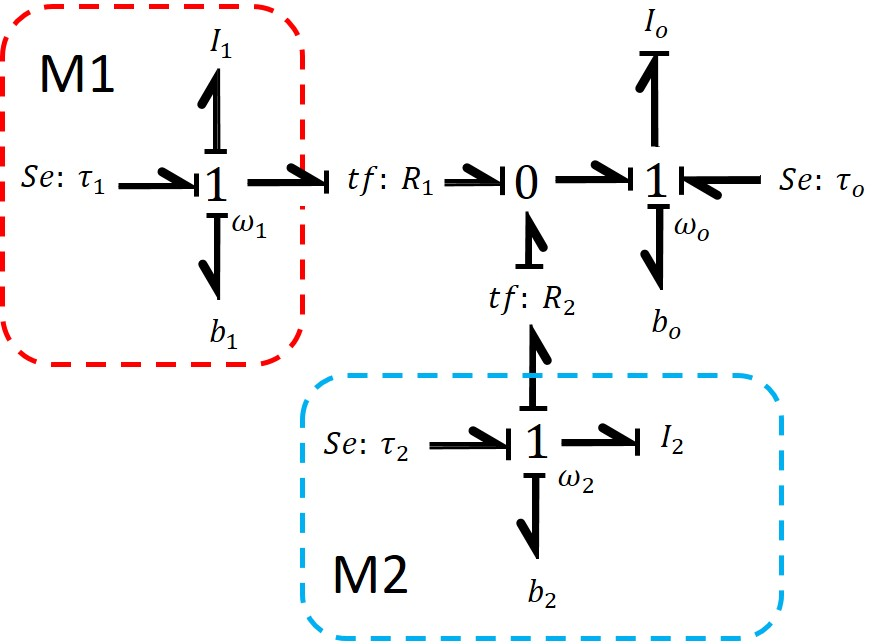
\includegraphics[width=0.65\textwidth]{dynamics_bond.jpg}
	\caption{Bond-graph dynamic model of a DSDM}
	\label{fig:dynamics_bond}
\end{figure}

Applying Newton's law on each ports yields the following equations of motions:
%
\begin{align}
\tau_{ext}  - e_o &= Z_o(s) w_o \\
\tau_{1}    - e_1 &= Z_1(s) w_1 \\
\tau_{2}    - e_2 &= Z_2(s) w_2
\end{align}
%
where $Z_i(s) = I_i s + b_i$ represents the mechanical impedance of the i-th ports. Note that the system is coupled due to the constraint given by eq. \eqref{eq:kinematic} and \eqref{eq:torque}, and that there is only two degrees of freedom among the three ports. Fig. \ref{fig:dynamics_block}, illustrate the coupled equations motion in block diagram form.
%
\begin{figure}[htp]
	\centering
		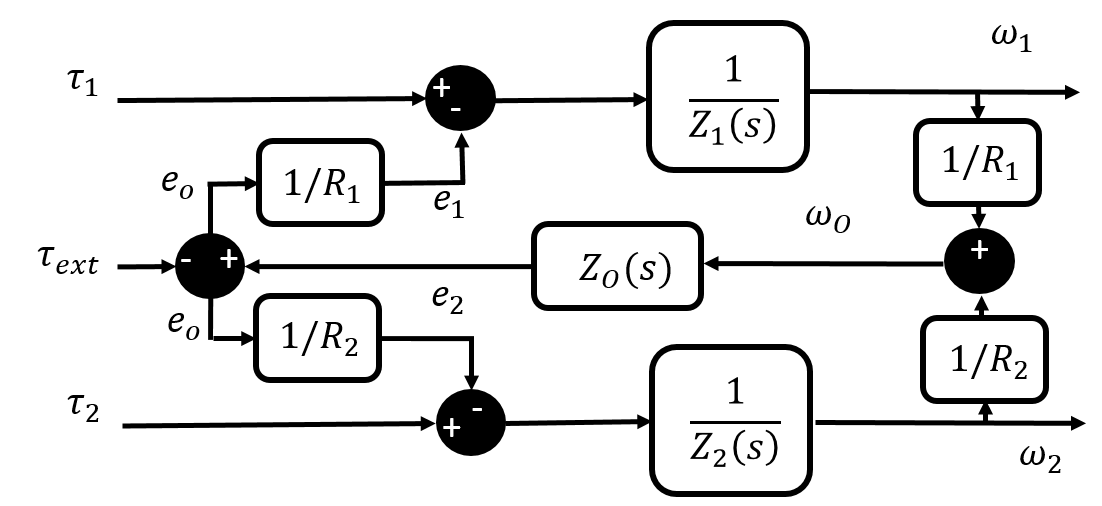
\includegraphics[width=0.70\textwidth]{dynamics_block.png}
	\caption{Dynamics of a DSDM illustrated with a block diagram}
	\label{fig:dynamics_block}
\end{figure}
%
It is then possible to eliminate one variable and express the dynamic as the following system of two equations:
%
\begin{align}
\left[
\begin{array}{c c c}
 1 & 0 & \frac{1}{R_1} \\
 0 & 1 & \frac{1}{R_2}
\end{array}
\right]
\left[
\begin{array}{l}
 \tau_{1} \\
 \tau_{2} \\
 \tau_{ext}
\end{array}
\right]
=
\left[
\begin{array}{c c}
 Z_1(s) + \frac{Z_0(s)}{R_1^2} & \frac{Z_0(s)}{R_1 R_2}        \\
 \frac{Z_0(s)}{R_1 R_2}        & Z_2(s) + \frac{Z_0(s)}{R_2^2} \\
\end{array}
\right]
\left[
\begin{array}{l}
w_1     \\
w_2     \\
\end{array}
\right]
\end{align}
% Alternative
%%
%\begin{align}
%\left[
%\begin{array}{c c c}
 %1 & 0 & \frac{1}{R_1} \\
 %0 & 1 & \frac{1}{R_2}
%\end{array}
%\right]
%\left[
%\begin{array}{l}
 %\tau_{1} \\
 %\tau_{2} \\
 %\tau_{ext}
%\end{array}
%\right]
%=
%\left[
%\begin{array}{c c}
%\frac{Z_o(s)}{R_1}  &   \scriptstyle Z_1(s)   \\
%\frac{Z_o(s)}{R_2}  \scriptstyle + R_2 Z_2(s) & \scriptstyle-\textstyle \frac{R_2}{R_1} \scriptstyle Z_2(s)   \\
%\end{array}
%\right]
%\left[
%\begin{array}{l}
%w_o     \\
%w_1     \\
%\end{array}
%\right]
%\end{align}
%
The equation of motion can then be rearranged in the standard manipulator equation form, using $ \left[
\begin{array}{c}
w_o \\ w_1 
\end{array}
\right] = \vec{w} = \vec{\dot{q}} $ as generalized coordinates:
%
\begin{align}
\underbrace{ 
\left[
\begin{array}{c c}
 \scriptstyle I_o + R_2^2 I_2           & \scriptstyle - \frac{R_2^2}{R_1} I_2       \\
 \scriptstyle - \frac{R_2^2}{R_1} I_2   & \scriptstyle I_1 + (\frac{R_2}{R_1})^2 I_2  \\
\end{array}
\right] }_{H}
\underbrace{ 
\left[
\begin{array}{l}
\dot{w}_o     \\
\dot{w}_1      \\
\end{array}
\right]}_{\vec{\ddot{q}}}
+
\underbrace{
\left[
\begin{array}{c c}
 \scriptstyle b_o + R_2^2 b_2           & \scriptstyle - \frac{R_2^2}{R_1} b_2       \\
 \scriptstyle- \frac{R_2^2}{R_1} b_2   & \scriptstyle b_1 + (\frac{R_2}{R_1})^2 b_2  \\
\end{array}
\right]
}_{D}
\underbrace{ 
\left[
\begin{array}{l}
w_o     \\
w_1      \\
\end{array}
\right]}_{\vec{\dot{q}}}
= \\
\underbrace{ 
\left[
\begin{array}{c c c}
 \scriptstyle 0 & \scriptstyle R_2              & \scriptstyle 1 \\
 \scriptstyle 1 & \scriptstyle -\frac{R_2}{R_1} & \scriptstyle 0
\end{array}
\right]}_{B}
\underbrace{
\left[
\begin{array}{l}
 \tau_{1} \\
 \tau_{2} \\
 \tau_{ext}
\end{array}
\right] }_{\vec{\tau}}
\label{eq:dsdm_manip}
\end{align}
%
The inverse of the inertia matrix is given by:
\begin{align}
H^{-1} = 
\frac{1}{I_o + I_1 R_1 ^2 + I_o \frac{ I_1 }{ I_2 } (\frac{R_1}{R_2})^2}
\left[
\begin{array}{c c}
1 + \frac{ I_1 }{ I_2 } (\frac{R_1}{R_2})^2  & R_1    \\
R_1 & \frac{ I_0 }{ I_2 } (\frac{R_1}{R_2})^2 + R_1^2 \\
\end{array}
\right]
\end{align}
%
The equations can be converted to linear state space form:
\begin{align}
\underbrace{ \vec{\dot{w}} }_{\dot{\vec{x}}}
 &= 
\underbrace{ \left[ -H^{-1} D \right] }_{F}
\underbrace{ \vec{w} }_{\vec{x}}
+ 
\underbrace{ \left[ H^{-1} B \right] }_{G}
\underbrace{ \vec{\tau} }_{\vec{u}}
\end{align}
%
Leading to the following after eliminating the external torque and the damping at each motor port for brevity:
\begin{align}
\left[
\begin{array}{c}
\dot{w_o}\\
\dot{w_1}
\end{array}
\right] &= 
F
\left[ \begin{array}{c}
w_o \\
w_1
\end{array} \right]+
G
\left[ \begin{array}{c}
\tau_1 \\
\tau_2
\end{array} \right] 
\label{eq:ss}
\\
\text{with} \quad 
F &=
\frac{1}{I_T}
\left[
\begin{array}{c c}
-b_T      &  0 \\
-R_1 b_o  &  0 \\
\end{array}
\right] \\
G &= 
\frac{1}{I_T}
\left[
\begin{array}{c c}
 R_1  &   R_1 \frac{R_1 I_1}{R_2 I_2}  \\
(R_1^2+\frac{R_1^2 I_o}{R_2^2 I_2})  &  - \frac{R_1 I_o}{R_2 I_2} \\
\end{array}
\right] \\
 I_T &=  \scriptstyle \left[   I_o + R_1^2 I_1 + \left( \frac{R_1}{R_2} \right)^2 \frac{I_1}{I_2} I_o \right]\\
 b_T &= \scriptstyle \left[ b_o + \left( \frac{R_1}{R_2} \right)^2 \frac{I_1}{I_2} b_o \right] 
\end{align}
%


\subsection{Inputs/Outputs equations}
\label{sec:out}

The variable of interest is the output $w_o$, and its dynamic can be expressed, going back to the Laplace domain by:
%
\begin{align}
\left[
 Z_1(s) Z_2(s) + \frac{Z_1(s) Z_o(s)}{R_2^2} + \frac{Z_2(s) Z_o(s)}{R_1^2}
\right] w_o(s) = \\
\left[
 \frac{Z_2(s)}{R_1}
\right] \tau_1(s)  + 
\left[
 \frac{Z_1(s)}{R_2}
\right] \tau_2(s)  + 
\left[
 \frac{Z_2(s)}{R_1^2} + \frac{Z_1(s) }{R_2^2}
\right] \tau_{ext}(s)
\label{eq:dsdm_output}
\end{align}

When the brake on M1 of the DSDM is locked, the output equation is reduced, by letting $Z_1(s) \rightarrow \infty$, to:
\begin{align}
\left[
 Z_o(s)  + R_2^2 Z_2(s)
\right] w_o(s) = 
\left[
R_2
\right] \tau_2(s)  + 
\tau_{ext}(s)
\label{eq:dsdm_output_HF}
\end{align}

When the brake is open, if the gear-ratio $R_2$ of M2 is large, the equation can be simplified. 
%
%, the behavior can be approximated. First eq. \eqref{eq:dsdm_output} is rearranged:
%\begin{align}
%\left[
%\scriptstyle Z_1(s) R_1^2 + \left(1 + \frac{Z_1(s) R_1^2 }{ Z_2(s) R_2^2} \right) Z_o(s)
%\right] w_o(s) = 
%\left[
%R_1
%\right] \tau_1(s)  + 
%\left[
%\scriptstyle R_1 \frac{R_1 Z_1(s)}{R_2 Z_2(s)}
%\right] \tau_2(s)  + 
%\left[
%\scriptstyle  1 + \frac{Z_1(s) R_1^2 }{ Z_2(s) R_2^2} 
%\right] \tau_{ext}(s)
%\label{eq:dsdm_output_HS}
%\end{align}
%
Assuming the reflected impedance of M1 is much smaller than that of M2, and neglecting motor side damping, the equation reduce to:
\begin{align}
\left[
Z_o(s)  + R_1^2 Z_1(s)
\right] w_o(s) &= 
\left[
R_1
\right] \tau_1(s)  + 
\left[
R_1 \frac{R_1 I_1}{R_2 I_2}
\right] \tau_2(s)  + 
\tau_{ext}(s) \\
&\text{if} \quad Z_1(s) R_1^2 << Z_2(s) R_2^2 
\quad \& \quad \frac{Z_1(s)}{Z_2(s)} = \frac{I_1}{I_2}
\label{eq:dsdm_output_HS}
\end{align}

During high-speed mode the behavior of the output is also dominated by a first-order linear behavior, but interestingly both input torques contributed to the motion through inertial coupling. Note that this differ from a serial architecture, in both case speed adds-up and effort is shared (0-type junction), but inertial properties are different.

\begin{align}
\text{High-speed mode: } \quad \left[ I_o + R_1^2 I_1 \right] \dot{w}_o +  \left[ b_o \right] \dot{w}_o  &= \left[ R_1 \right] \tau_1 + \left[ R_1 \frac{R_1 I_1}{R_2 I_2} \right] \tau_2 
\label{eq:dsdm_output_HSw0} \\
\text{High-force mode: } \quad \left[ I_o + R_2^2 I_2 \right] \dot{w}_o +  \left[ b_o \right] \dot{w}_o  &= \left[ R_2 \right] \tau_2 
\label{eq:dsdm_output_HFw0}
\end{align}

Note that, if DSDM would be used on multi-DoF robots, the left-hand side of equations \eqref{eq:dsdm_output_HSw0} and \eqref{eq:dsdm_output_HFw0} would be more complex: including coupled inertial effects, gravitation forces and others. However, the right-hand side of the equation would stay the same: the motor torques transmission gains would not be affected. Also, although neglected in \eqref{eq:dsdm_output_HSw0} and \eqref{eq:dsdm_output_HFw0}, motor damping could be reintroduce easily by substituting motor torque $\tau_i$ with the effective torque $\tau_i - b_i w_i$ since those forces are collocated. 

\subsection{Hybridness due to Discrete Operating Modes and Impacts}

Fig. \ref{fig:operatingmodes} illustrates the two different discrete modes of the system. During high-force mode, when the brake is engaged, the actuator only has a single DoF and control input and the behavior is described by differential equations $f_1$. During high-speed mode, when the brake is open, the actuator has two DoF and two control inputs and the behavior is described by differential equations $f_1$. As illustrated, at the moment the brake is opened or closed, the discrete mode and the states also instantaneously change, according to some mapping (up-shift $h_u$ and down-shift $h_d$). It is also possible that during operation the actuator output hit an object leading to an impulsive behavior. This behavior is modeled by reset map $h_1$ and $h_2$. This hybrid model capture all the possibles behavior in the course of normal operation.

\begin{figure}[H]
	\centering
		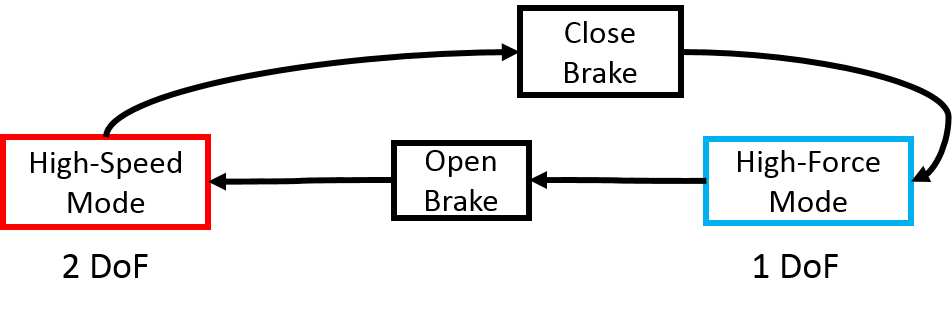
\includegraphics[width=0.95\textwidth]{operating_modes.png}
	\caption{Discrete operating modes of the actuators TODO: update with jump map}
	\label{fig:operatingmodes}
\end{figure}


Table \ref{tab:hybrid} outline each mapping given at Fig. \ref{fig:operatingmodes} to corresponding equations.

\begin{table}[htbp]
	\centering
	\caption{Hybrid model: Continous equations and discrete jump maps}	% Table caption must be placed on top of the table %
		\begin{tabular}{ c c c c }
				\hline \hline
				Situation           & Discrete Mode     & Mapping   & Equation of motions \\
				\hline \hline
				\multicolumn{4}{c}{ Continuous differential equations }\\
        \hline
			   High-Force Mode    & $k=1$             & $\dot{\vec{w}} = f_1(\vec{w})$  & given by eq. \eqref{eq:dsdm_output_HF} \\
				 High-Speed Mode    & $k=2$             & $\dot{\vec{w}} = f_2(\vec{w})$  & given by eq. \eqref{eq:ss}             \\
				\hline
				\multicolumn{4}{c}{ Discrete gear-shift jump maps }\\
				\hline
				 Up-shift           & $k:1\rightarrow2$  & $\vec{w}^+= h_u(\vec{w}^-)$  &  given by eq. \eqref{eq:upshiftmap}\\
				 Down-shift         & $k:2\rightarrow1$  & $\vec{w}^+= h_d(\vec{w}^-)$  &  given by eq. \eqref{eq:downshiftmap_ideal}\\
				\hline
				\multicolumn{4}{c}{ Output impact jump maps }\\
				\hline
				 Impact during HF   & $k:1\rightarrow1$  & $\vec{w}^+= h_1(\vec{w}^-)$  &  \\
				 Impact during HS   & $k:2\rightarrow2$  & $\vec{w}^+= h_2(\vec{w}^-)$  &  \\
		    \hline \hline
        \end{tabular}		
	\label{tab:hybrid}
\end{table}


%%%%%%%%%%%%%%%%%%%%%%%%%%%%%%%%%%%%%%%%%%%%%%%%%%%%%%%%%%%%%%%%%%%%%%%%%%%%%%%%%%%%%%%%%%%%%%%%%%%%%%%%%%%%%

\subsection{Gear-shift events}

\subsubsection{Up-Shift}

During high-force mode, the single DoF is described by the variable $w_o$. Opening the brake release a constraint in the system and do not lead to any impulsive behavior. M1 rotor is simply suddenly free to move starting from rest. The mapping is thus giving by:
\begin{align} 
\left[
\begin{array}{c}
w_o^+ \\ w_1^+
\end{array}
\right] = h_u( w_o^- ) = 
\left[
\begin{array}{c}
w_o^- \\ 0
\end{array}
\right]
\label{eq:upshiftmap}
\end{align}



\subsubsection{Down-shift}

For a down-shift the system goes from 2-DoF to 1-DoF, hence the sudden addition of a constraint (brake locked) can lead to an impulsive behavior. However, as it will be discuss in the next section, the controller will always make sure that M1 is at zero velocity before engaging the brake in order to avoid this impulsive behavior. 

%\paragraph{Ideal case}

In normal operation, M1 velocity will be brought to zero before engaging the brake and the mapping is thus smooth and given by:
%
\begin{align} 
w_o^+ 
 = h_d( \vec{w}^- ) = 
w_o^- \quad \text{if} \quad w_1^-=0
\label{eq:downshiftmap_ideal}
\end{align}


%\paragraph{Bad synchronization}
%
If the brake would be engaged with non-zero velocity, TODO
\begin{align} 
w_o^+ 
 = h_d( \vec{w}^- ) = 
w_o^- + TODO(w_1^-)
\label{eq:downshiftmap_ideal}
\end{align}



%%%%%%%%%%%%%%%%%%%%%%%%%%%%%%%%%%%%%%%%%%%%%%%%%%%%%%%%%%%%%%%%%%%%%%%%%%%%%%%%%%%%%%%%%%%%%%%%%%%%%%%%%%%%%

\subsection{Impacts}
\label{sec:model_impact}

\subsubsection{High-speed mode impact}

During a contact, impulsive forces can create a sudden change of velocity. Hence, if a DSDM actuator is used on a robotic system making contact with objects, its internal velocities will suddenly change, as a function of the full dynamic of the robot and the contact situation:
%
\begin{align}
\left[
\begin{array}{c}
w_0^+ \\
w_1^+ \\
\end{array}
\right] = 
\left[
\begin{array}{c}
w_0^- \\
w_1^- \\
\end{array}
\right] +
\vec{h}( \vec{q} , \vec{\dot{q}} , J_c )
\end{align}
%
where $\vec{h}$ can be a complex mapping involving high-dimensional dynamic and constraints. However, since there is no impulsive force on the motor side, the effect of the contact, from the actuator point-of-view, can be reduce to a impulse torque $\tau_c$ applied to the output of the actuator, leading to:
%
\begin{align}
\left[
\begin{array}{c}
w_0^+ \\
w_1^+ \\
\end{array}
\right] = 
\left[
\begin{array}{c}
w_0^- \\
w_1^- \\
\end{array}
\right] +
H^{-1} \left[
\begin{array}{c}
1 \\
0 \\
\end{array}
\right] \int{\tau_c dt}
\end{align}
%
If the reflected inertia of M2 is much greater than that of M1 ($R_2^2 I_2 >> R_1^2 I_1 $), than the impulsive reaction is expressed by:
%
\begin{align}
\left[
\begin{array}{c}
w_0^+ \\
w_1^+ \\
\end{array}
\right] = 
\left[
\begin{array}{c}
w_0^- \\
w_1^- \\
\end{array}
\right] +
\frac{ \int{\tau_c dt} }{ I_o + I_1 R_1^2} 
\left[
\begin{array}{c}
1 \\
R_1 \\
\end{array}
\right] 
\end{align}
%
Hence, M2 velocity will be unchanged and the velocity discontinuity of the output is transmitted directly to M1 during an impact:
%
\begin{align}
\Delta w_o  &= w_o^+ - w_o^- = \frac{ \int{\tau_c dt} }{ I_o + I_1 R_1^2}  \\
\Delta w_1  &= w_1^+ - w_1^- = R_1 \Delta w_o \\
\Delta w_2  &= w_2^+ - w_2^- =  0
\label{eq:dsdm_impact_gen_delta_w1}
\end{align}


\subsubsection{High-force mode impact}

TODO

%\begin{figure}[H]
	%\centering
		%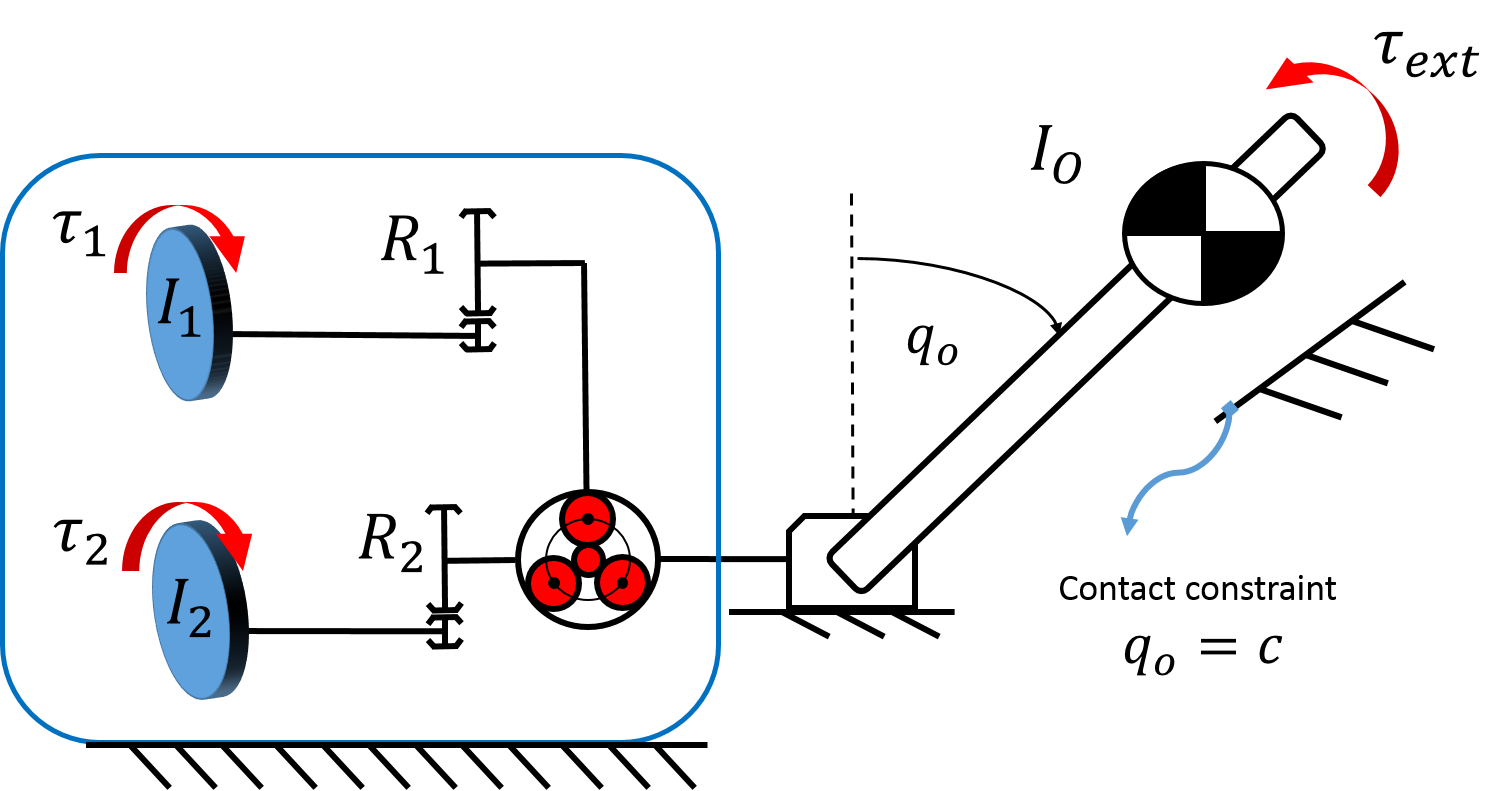
\includegraphics[width=0.70\textwidth]{dsdm_impact_model.png}
	%\caption{DSDM actuator impact model}
	%\label{fig:dsdm_impact_model_1}
%\end{figure}

%
%\paragraph{Example}
%Fig.\ref{fig:dsdm_impact_model_1} illustrates a simple impact scenario with a single DSDM actuator. The equation of motion previous introduced (eq. \eqref{eq:dsdm_manip}) can describe this situation. However here, displacement variables corresponding to angles of rotation of the output and M1, ignorable coordinates for an unconstrained scenario, are introduced:
%%
%\begin{align}
%\vec{q} = \left[ \begin{array}{c} 	q_0 \\ q_1 \end{array} \right] \quad
%\vec{\dot{q}} = \left[ \begin{array}{c} 	w_0 \\ w_1 \end{array} \right]
%\label{eq:dsdm_impact_q}
%\end{align}
%%
%Then the contact constraint is expressed in the standard form (see section \ref{sec:contact}):
%%
%\begin{align}
%\phi( \vec{q} )       &= q_0 - c = 0 \\
%\dot{\phi}( \vec{q} ) &= J_c\vec{\dot{q}} =  w_0 = 0 \\
%J_c                   &= \frac{d \phi}{d\vec{q}} = \left[ \begin{array}{c c} 1 & 0 \end{array} \right]
%\label{eq:dsdm_impact_const}
%\end{align}
%%
%Then it is assumed that the impact is completely inelastic and again, for simplicity that $R_2^2 I_2 >> R_1^2 I_1$. Solving for the impact force using eq.\eqref{eq:manipulator_impact_force} lead to:
%%
%\begin{align}
%\int{  \tau_c dt } &= - \left( J_c H^{-1} J_c^T \right)^{-1}  J_c \vec{\dot{q}}^- = -(I_0 + I_1 R_1^2) w_o^-
%\label{eq:dsdm_impact_force}
%\end{align}
%%
%and the resulting change in velocities during the impact are thus:
%\begin{align}
%\Delta w_o  = - w_o^- \quad  \Delta w_1  = - R_1 w_o^-  \quad  \Delta w_2  = 0
%\label{eq:dsdm_impact_res}
%\end{align}






%%%%%%%%%%%%%%%%%%%%%%%%%%%%%%%%%%%%%%%%%%%%%%%%%%%%%%%%%%%%%%%%%%%%%%%%%%%%%%%%%%%%%%%%%%%%%%%%%%%%%%%%%%%%%%%%%%%%%%%%%%%%

\subsection{Nullspace of the system during high-speed mode}

\subsubsection{Kinematic}

During high-speed mode, from the kinematic input-output view point, the DSDM actuator has one redundant degree of freedom. In other words, there is an infinite number of combinations of $w_1$ and $w_2$ producing the same output speed $w_0$, from eq.\eqref{eq:kinematic}:  
%
\begin{align}
w_o
 = 
\left[
\begin{array}{c c}
\frac{1}{R_1} & \frac{1}{R_2}
\end{array}
\right]
\left[
\begin{array}{c}
w_1 \\
w_2 \\
\end{array}
\right]
\end{align}
%
A vector perpendicular to the above coefficient vector forms the null space of the DSDM actuator system. Any input combination in this direction produces zero output speed:
%
\begin{align}
\left[
\begin{array}{c}
w_1 \\
w_2 \\
\end{array}
\right]=
\underbrace{\left[
\begin{array}{c}
1 \\
-R_2/R_1 \\
\end{array}
\right]}_{\text{Nullspace Projection}}
u  \; \rightarrow \;
w_0 = 0 \quad \forall u \in \Re
\label{eq:kinematicnullspace}
\end{align}
%

\subsubsection{Dynamic}

Interestingly, a similar expression can be obtained for the dynamics of the output in response to electromagnetic torque inputs, from the first line of eq.\eqref{eq:ss}:
%
\begin{align}
I_T \dot{w}_o +
b_T  w_o
=&
\left[ \begin{array}{c c}
R_1 & R_1 \frac{R_1 I_1}{R_2 I_2}
\end{array} \right]
\left[ \begin{array}{c}
\tau_1 \\
\tau_2
\end{array} \right]
\label{eq:output}
\end{align}
% 
Hence, there is a one degree of freedom space of inputs $\tau_1$ and $\tau_2$ that do not affect the output:
\begin{align}
\left[ \begin{array}{c}
\tau_1 \\
\tau_2
\end{array} \right]
 = 
\underbrace{\left[ \begin{array}{c}
I_1 \\
-\frac{R_2 }{R_1 }  I_2
\end{array} \right]}_{\text{Nullspace Projection}} u
\; \rightarrow \;
I_T \dot{w}_o +
b_T  w_o = 0 \quad \forall u \in \Re
\label{eq:dyn_null_proj}
\end{align}


\subsection{Equivalence to a two-speed transmission}

Assuming a only M1 is used during high-speed mode and only motor M2 is used during high-force mode ( i.e. the control input is either $\tau_1$ or $\tau_2$ according to the mode) and additionally if the two motors are identical, then the behavior is equivalent to a motor with a two-speed transmission. 

From an outer-loop point of view, if the commanded torque to the DSDM actuator is routed this way:

\begin{align}
\text{High-speed mode: }\tau_1 = \tau \quad \tau_2 = 0    \quad \text{if} k=0 \\
\text{High-force mode: }\tau_1 = 0    \quad \tau_2 = \tau \quad \text{if} k=1
\end{align}

Then the equation of motions for each operating mode, eq. \eqref{eq:dsdm_output_HSw0} and eq. \eqref{eq:dsdm_output_HFw0},  are simplifyied to:

\begin{align}
\text{High-speed mode: } \quad \left[ I_o + R_1^2 I_1 \right] \dot{w}_o +  \left[ b_o \right] w_o  &= \left[ R_1 \right] \tau 
\label{eq:dsdm_output_R1} \\
\text{High-force mode: } \quad \left[ I_o + R_2^2 I_2 \right] \dot{w}_o +  \left[ b_o \right] w_o  &= \left[ R_2 \right] \tau 
\label{eq:dsdm_output_R2}
\end{align}

and they can be reduced the same structure :

\begin{align}
\left[ I_o + R_k^2 I_k \right] \dot{w}_o +  \left[ b_o \right] w_o  &= \left[ R_k \right] \tau \quad k \in {1,2}
\label{eq:dsdm_output_R} 
\end{align}

where only the gear-ratio is different. This would thus be equivalent to the system illustrated at Fig. XX, and also correspond to a single motor equipped with a two speed transmission (if  $I_1 = I_2$).



\newpage

\section{Control algorithms}

\begin{figure}[H]
	\centering
		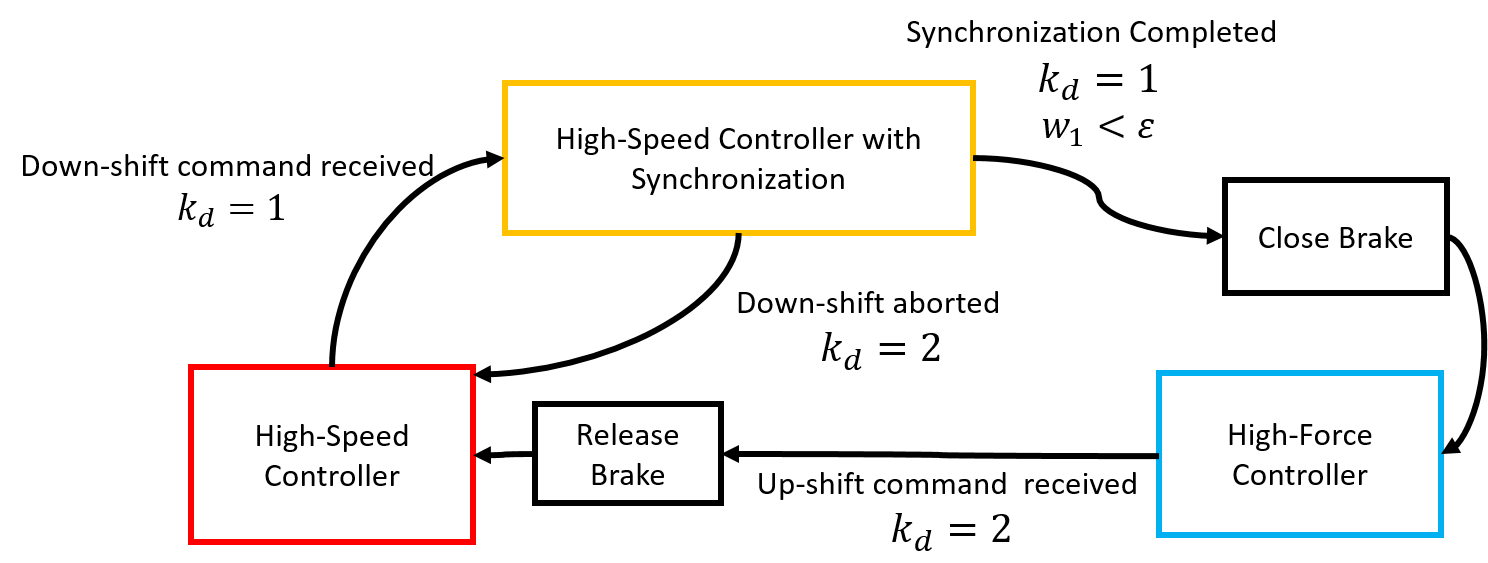
\includegraphics[width=0.90\textwidth]{operating_modes_ctl.png}
	\caption{State machine of discrete control modes}
	\label{fig:automaticflow}
\end{figure}

\begin{figure}[H]
	\centering
		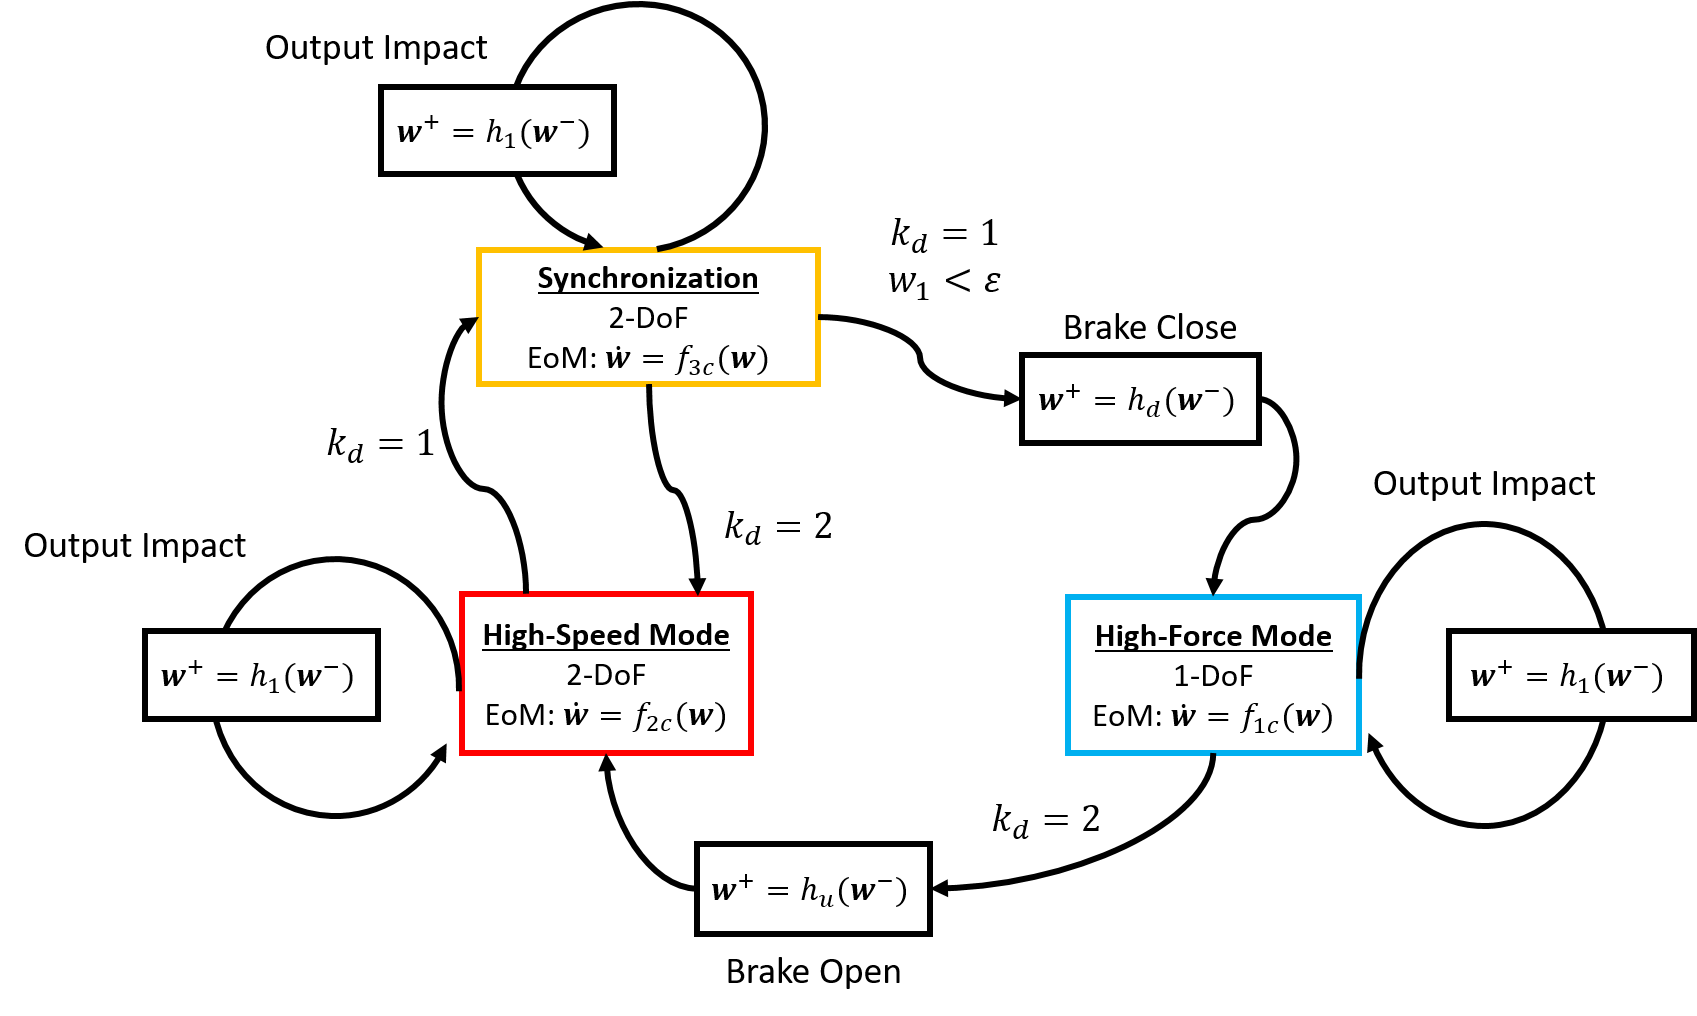
\includegraphics[width=0.90\textwidth]{operating_modes_CL.png}
	\caption{Hybrid Behavior in Closed-loop}
	\label{fig:hybrid_closedloop}
\end{figure}

\subsection{High-force mode controller}

During high-force mode, the actuator behaves like a regular geared EM motor and standard control schemes can be used. %Fig. \ref{fig:HF_loop} illustrates the high-force mode control laws for the case when a high-level control loop specify output torque and operating mode.


\subsection{High-speed mode controller}

During high-speed mode, with a small reduction ratio $R_1$ (high transparency transmission), the DSDM actuator can be controlled like a direct drive motor: controlling M1 current lead to almost direct control of the output torque. Moreover, exploiting the nullspace, a secondary objective can be brought into the system without influencing the output torque. In case the first motor is overloaded, for example, the second motor can reduce the load by projecting inputs through the null space, producing no effect upon the output, but changing the proportion of the two input commands. The secondary controller can be used not only for load balancing but also for minimizing power consumption, avoiding speed saturation of M1, etc. Note that the nullspace projection vector, see eq.\eqref{eq:dyn_null_proj}, depends only on parameters associated with the motors. Therefore, it is possible to project the secondary controller inputs on the output nullspace even if the output dynamic parameters that include the load inertia and damping are unknowns. 

Fig. \ref{fig:HS_loop} and Fig. \ref{fig:HF_loop} show DSDM control algorithms implemented as intermediary control loops between hardware and high-level commands. The high-speed controller tracks a received desired torque by controlling the current in M1, and can also optionally track a secondary objective without affecting the main-loop, by projecting the secondary input into the nullspace of the main-loop. The high-force controller directly convert a received desired torque to a current set-point for M2.


\subsection{Fast and Seamless Transitions (gear-shift)}

This section addresses transition control between the two discrete operating modes. Fig. \ref{fig:automaticflow} show the state machine used to transit between the different necessary control mode.


\paragraph{Up-shift: From high-force mode to high-speed mode}
In this case, the transition is simple because the system goes from 1 DoF to 2 DoF. The locking brake can be released anytime, M1 is then instantaneously freed and the controller can immediately switch to the high-speed control mode.
%

\paragraph{Down-shift: From high-speed mode to high-force mode}
In this case, the transition is harder because the system goes from 2 DoF to 1 DoF, and some synchronization work is needed. M1 speed $w_1$ must be brought to zero so that the locking brake can be engaged smoothly without any impact. Hence, as illustrated at Fig. \ref{fig:automaticflow}, when it is decided to engage high-force mode, and intermediary synchronization control mode is needed. Two algorithms, a kinematic and a dynamic approach, can be considered. 

%\paragraph{Kinematic algo}
The kinematic control aglorithm assumes local high gain velocity feedback controls for the individual motors. Hence velocities $w_1$ and $w_2$ can be treated as control inputs. Using the nullspace projection vector from eq.\eqref{eq:kinematicnullspace}, the kinematic control law can be written as 
%
\begin{align}
\left[
\begin{array}{c}
w_1 \\
w_2 \\
\end{array}
\right]=
\underbrace{\left[
\begin{array}{c}
1 \\
-R_2/R_1 \\
\end{array}
\right]}_{\text{Nullspace Projection}}
u_1 + 
\left[
\begin{array}{c}
0 \\
R_2 \\
\end{array}
\right] u_0
\label{eq:kinematicsys}
\end{align}
%
leading to
%
\begin{align}
w_o = u_0 \quad \text{with} \quad w_1 = u_1
\end{align}
%
Therefore during transitions, using $u_1$ velocity $w_1$ can be driven to zero, while fully controlling the output velocity using $u_0$. The kinematic control law is valid only when high fidelity velocity controls are available. Alternatively the dynamic control algorithm does not require this. 

%\paragraph{Dynamic algo}
As illustrated in Fig. \ref{fig:down_loop}, while running the general high-speed controller, a braking law for $w_1$ can be used in parallel as the secondary controller projected on the output nullspace:
\begin{align}
\left[ \begin{array}{c}
\tau_1 \\
\tau_2
\end{array} \right]
 = 
\underbrace{\left[ \begin{array}{c}
I_1 \\
-\frac{R_2 }{R_1 }  I_2
\end{array} \right]}_{\text{Nullspace Projection}} \underbrace{-C w_1}_{\text{Braking Law}} + 
\left[ \begin{array}{c}
1 \\
0 
\end{array} \right]  \tau_d
\label{eq:syncrhonization_ctl}
\end{align}
leading to independent output dynamics controlled with $\tau_d$:
\begin{align}
I_T \dot{w}_o +
b_T  w_o
=& \, R_1 \tau_d  
\end{align}
and a $w_1$ closed-loop dynamic converging exponentially to zero if the synchronization gain $C$ is large:
\begin{align}
 %\dot{w}_1 = -C w_1 + f(w_o,\tau_d) %\scriptstyle \frac{R_1 b_o}{I_T} \textstyle w_o
 \dot{w}_1 = -C w_1 + \underbrace{\left[\frac{R_1^2}{I_T} + \frac{R_1^2 I_o}{R_2^2 I_2 I_T} \right] \tau_d - \left[\frac{R_1 b_o}{I_T}\right] w_o }_{\text{Undesirable coupling from main loop}}
\end{align}

Hence, the output is not influenced by the braking law due to orthogonality, and is still controlled using the desired torque $\tau_d$ determined by the high-speed mode controller. On the other hand, $w_1$ is directly influenced by the braking law but also by the output speed and the desired output torque $\tau_d$. Mathematically, it would be possible to also fully uncouple $\dot{w}_1$ equation, but the control law would not be practical in the scenario of $R_1<<R_2$ when considering torque and speed saturations. Increasing the gain $C$ will lead to faster braking of $w_1$, however motor torque will saturate if the gain is too large. A large synchronization gain $C$ can still be used for faster braking at a cost of deviation from the desired torque $\tau_d$. There is thus a trade-off in practice, passed the torque saturation point, between fast braking of $w_1$ for fast transition and high-fidelity output torque control. Also the synchronization gain can be a complex compensator, for instance a PI ( $C(s) = k_p + \frac{k_i}{s}$ ), for better rejection of disturbances coming from the main loop coupling. 


\subsection{Predictive algorithm for fast down-shifts after a contact}

This section described a control scheme where the velocity of the internal DoF is adjusted beforehand when an impact is expected, so that impact forces bring M1 velocity close to zero, allowing for fast down-shift transitions. This is aimed at situation like a leg approaching the ground with high-speed mode, then making contact with the ground and transitioning to high-force mode to bear the weight of the robot.


%\paragraph{Kinematic algo}
Rearranging the results of section \ref{sec:model_impact} to express the two variables of interest (approaching speed $w_0^-$ and M1 velocity after the impact $w_1^+$), as a function of controllable inputs (from a kinematic point of view), lead to:
%
\begin{align}
\left[ \begin{array}{c} w_0^- \\ w_1^+ \end{array} \right] &= \Bigg[ \begin{array}{c c} \frac{1}{R_1} & \frac{1}{R_2}\\ 1 & 0 \end{array} \Bigg] \left[ \begin{array}{c} w_1^- \\ w_2^- \end{array} \right] + \left[ \begin{array}{c} 0 \\ R_1 \frac{\int{\tau_c dt}}{I_o + I_1 R_1^2} \end{array} \right]
\label{eq:dsdm_impact_approx_sol}
\end{align}
%
Hence it is possible to set both motor velocities so that the approaching speed and after impact M1 velocity can be set arbitrarily and independently using the nullspace, by determining velocity set-points as:
%
\begin{align}
\left[ \begin{array}{c} w_1^- \\ w_2^- \end{array} \right] &= \Bigg[ \begin{array}{c} R_1 \\ 0  \end{array} \Bigg] u_0  + 
\underbrace{ \left[ \begin{array}{c} 1 \\ -\frac{R_2}{R_1} \end{array} \right]}_{\text{Nullspace projection}}
 \left( u_1 - R_1 \frac{\int{\tau_c dt}}{I_o + I_1 R_1^2} \right) 
\end{align}
%
leading to
%
\begin{align}
 w_o^- = u_0 \quad \text{and} \quad w_1^+ = u_1
\end{align}
%
Therefore, if an impact is expected and the upcoming impulsive impact reaction $\int{\tau_c dt}$ can be computed, using this control law lead to independent control of the approaching speed of the actuator output $w_o^-$, which would be used for the primary objective (for instance making contact with the object at the right place and time), and resulting velocity of M1 after the impact $w_1^+$, which would be set to zero to allow for instantaneous down-shift.

%\paragraph{Dynamic algo}
%
Alternatively, as for the braking law used for synchronization during the down-shift process, this problem can be approached from a dynamic point of view. A desired velocity for M1 is defined has a function of the expected impulsive contact reaction:
%
\begin{align}
w_{1,d}  = - R_1 \frac{\int{\tau_c dt}}{I_o + I_1 R_1^2}
\label{eq:dsdm_impact_gen_delta_w1}
\end{align}
%
Then, while using the regular high-speed controller to control the output, the secondary objective loop can be used to track M1 velocity set-point $w_{1,d}$ in the nullspace. This is analogous to the synchronization controller of eq. \eqref{eq:syncrhonization_ctl} but with a non-zero set-point for M1:
%
\begin{align}
\left[ \begin{array}{c}
\tau_1 \\
\tau_2
\end{array} \right]
 = 
\underbrace{\left[ \begin{array}{c}
I_1 \\
-\frac{R_2 }{R_1} I_2 
\end{array} \right]}_{\text{Nullspace Projection}} \underbrace{C (w_{1,d} -  w_1)}_{\text{Speed controller}} + 
\left[ \begin{array}{c}
1 \\
0 
\end{array} \right]  \underbrace{ \tau_d }_{\text{Main Loop}}
\end{align}
%
As discussed before, this will lead to independent output dynamics controlled with $\tau_d$ which would be used by the main robot control loop:
\begin{align}
I_T \dot{w}_o +
b_T  w_o
=& \, R_1 \tau_d  
\end{align}
and a $w_1$ closed-loop dynamic converging exponentially to $w_{1,d}$ if the synchronization gain $C$ is large:
\begin{align}
 %\dot{w}_1 = -C w_1 + f(w_o,\tau_d) %\scriptstyle \frac{R_1 b_o}{I_T} \textstyle w_o
 \dot{w}_1 = C \left( w_{1,d} - w_1 \right) + \underbrace{\left[\frac{R_1^2}{I_T} + \frac{R_1^2 I_o}{R_2^2 I_2 I_T} \right] \tau_d - \left[\frac{R_1 b_o}{I_T}\right] w_o }_{\text{Undesirable coupling from main loop}}
\end{align}

If the velocity controller is able to track the velocity set-point and the collision is perfectly predicted, then immediately after the impact, M1 velocity will be zero:
%
\begin{align}
w_1^+ =  w_1^- + \Delta w_1 = w_{1,d}  + R_1 \frac{\int{\tau_c dt}}{I_o + I_1 R_1^2} \approx 0
\label{eq:dsdm_impact_vel}
\end{align}
%
Hence, it would be possible to engaged the brake and switch to high-force mode almost instantaneously. In practice, because of speed saturation it won't always be possible to perfectly track the desired speed $w_{1,d}$ in the nullspace, or to perfectly predict the contact impulse $\int{\tau_c dt}$. However, by running this control scheme and bringing $w_1^+$ as close as possible to zero, gear-shift will nonetheless be achieved faster because synchronization error will be smaller at the start of the down-shift process.

\begin{figure}[p]
	\centering
		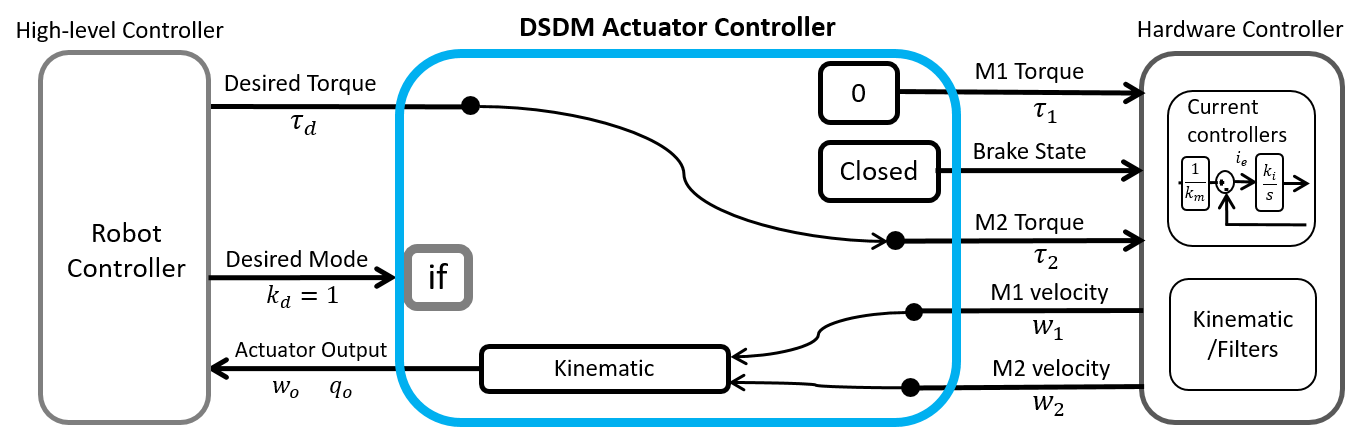
\includegraphics[width=0.95\textwidth]{HF_ctl.png}
	\caption{High-Force Mode Controller}
	\label{fig:HF_loop}
\end{figure}

\begin{figure}[p]
	\centering
		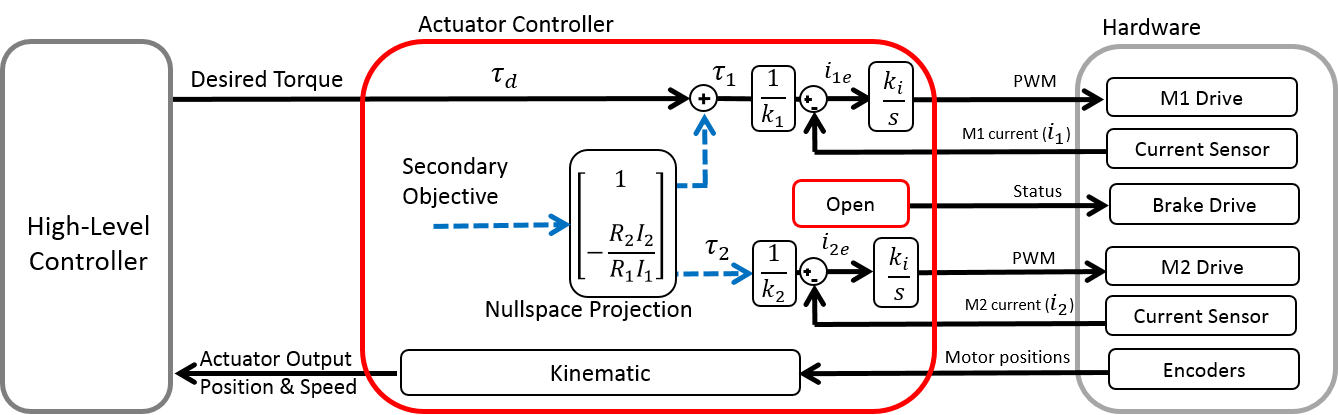
\includegraphics[width=0.95\textwidth]{HS_ctl.png}
	\caption{High-Speed Mode: Generic Controller}
	\label{fig:HS_loop}
\end{figure}

\begin{figure}[p]
	\centering
		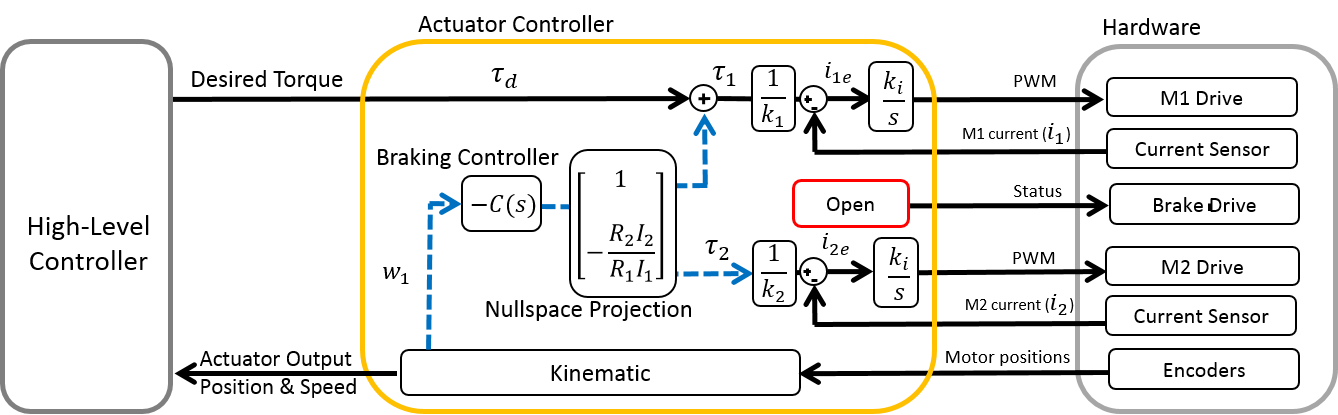
\includegraphics[width=0.95\textwidth]{down_ctl.png}
	\caption{High-Speed Mode: Synchronization controller}
	\label{fig:down_loop}
\end{figure}

\begin{figure}[p]
	\centering
		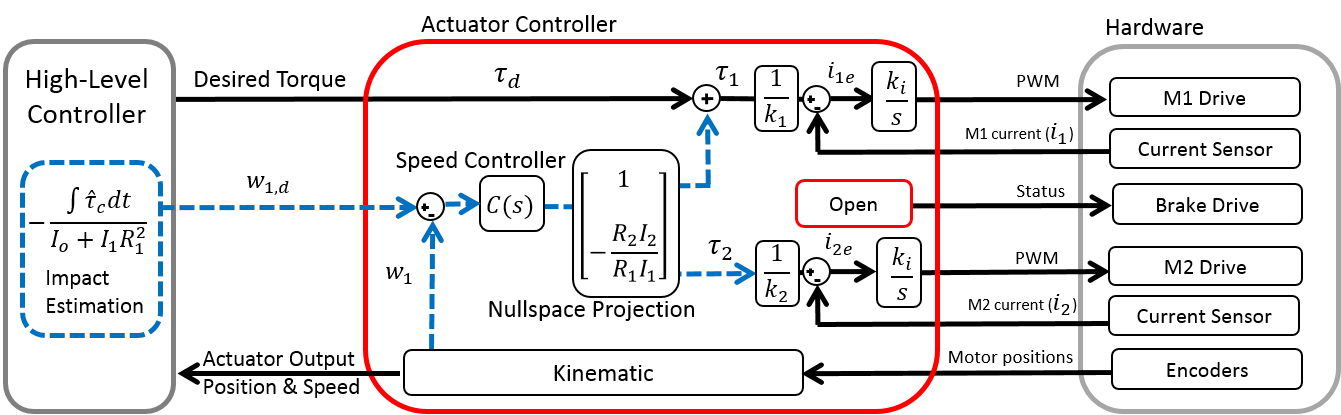
\includegraphics[width=0.95\textwidth]{imp_ctl.png}
	\caption{High-Speed Mode: Impact Preparation Controller}
	\label{fig:imp_loop}
\end{figure}

%\section{Experimental Validation}

\newpage

\section{Experimental Results}
\label{sec:dsdm_exp}

This section presents experimental results with the DSDM prototype illustrated at Fig. \ref{fig:dsdm_proto}. Refer to Chapter \ref{sec:ExperimentalValidation} for information regarding mecanical design and control implementation.

\subsection{DSDM Dynamic Behavior}

%\begin{figure}[H]
	%\centering
		%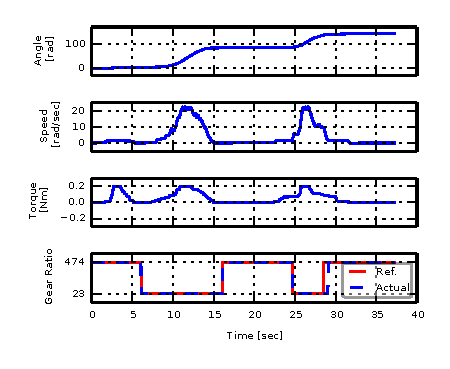
\includegraphics[width=0.95\textwidth]{dsdm_manual_all.pdf}
	%\caption[DSDM actuator torque control]{DSDM actuator with torque and mode commands set from a joystick }
	%\label{fig:dsdm_manual_all}
%\end{figure}
%
%\begin{figure}[H]
	%\centering
		%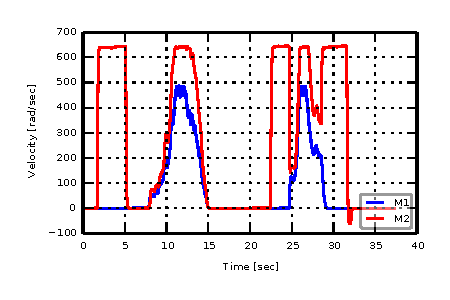
\includegraphics[width=0.95\textwidth]{dsdm_manual_motors.pdf}
	%\caption[DSDM actuator torque control]{DSDM actuator with torque and mode commands set from a joystick: Motors velocity }
	%\label{fig:dsdm_manual_motors}
%\end{figure}

Fig. \ref{fig:dsdm_manual_shift} gives an overview of how a DSDM actuator works. Before $t=2.5$, the brake is engaged and only M2 is used to drive the output. When is brake is engaged, the DSDM is in high-force mode and the effective gear-ratio is 474. At $t=2.5$, the brake is released and M1 start contributing to the motion. Releasing the brake will be referred to as an up-shift. Between $t=2.5$ and $t=6.5$, the brake is open, both motor contribute to the output speed; the DSDM is in high-speed mode and the effective gear-ratio is 23. At between $t=6.5$, a down-shift is manually commanded. Between $t=6.5$ and $t=7$, the synchronization controller then apply torques to brake M1 to zero speed and the brake is engaged at $t=7$ when M1 speed is detected to be null. This process of braking M1 and then engaging the brake will be referred as a down-shift.

\begin{figure}[htp]
	\centering
		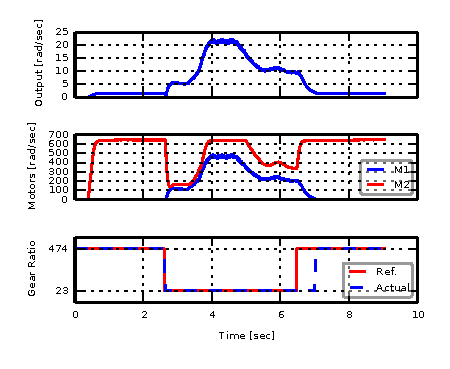
\includegraphics[width=0.75\textwidth]{dsdm_manual_shift.pdf}
	\caption[DSDM behavior overview]{DSDM actuator with torque and mode commands set from a joystick}
	\label{fig:dsdm_manual_shift}
\end{figure}

Fig. \ref{fig:dsdm_position_tracking} shows the DSDM tracking postion set-points with PD controllers. This experiment illustrates that the high-force mode is slow and with a highly damped behavior, while the high-speed mode is fast and with a under-damped second order behavior. 

\begin{figure}[htp]
	\centering
		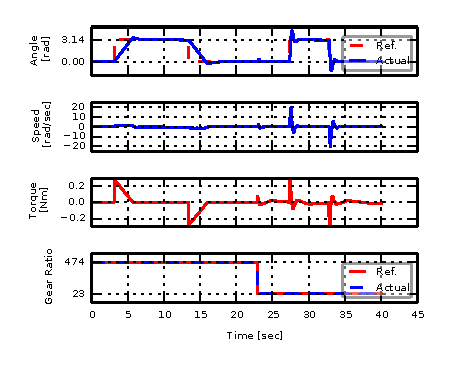
\includegraphics[width=0.75\textwidth]{dsdm_position_tracking.pdf}
	\caption[DSDM actuator position control]{DSDM actuator tracking position commanded from a joystick }
	\label{fig:dsdm_position_tracking}
\end{figure}


Fig. \ref{fig:dsdm_speed_tracking} shows the DSDM tracking speed set-points with PI controllers. Note that the noisy behavior during high-speed mode is only due to an implementation limitation: at low speed there is a quantization problem as their is a small amounts of encoder ticks per control loop interval. 


\begin{figure}[htp]
	\centering
		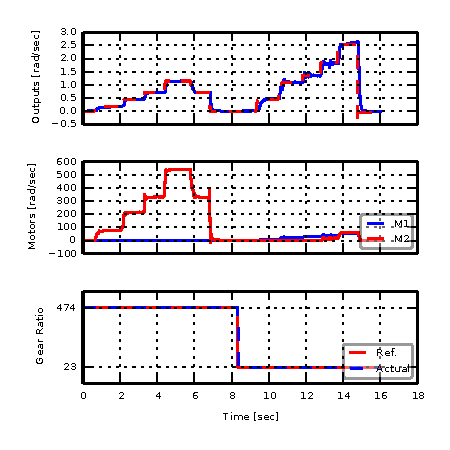
\includegraphics[width=0.75\textwidth]{dsdm_speed_tracking.pdf}
	\caption[DSDM actuator velocity control]{DSDM actuator tracking output velocity commanded from a joystick }
	\label{fig:dsdm_speed_tracking}
\end{figure}


\subsection{Nullspace}

Fig. \ref{fig:dsdm_nullspace} illustrates the internal DoF of DSDM actuators. Here the DSDM tracks a constant output speed while motor speeds are varied by projecting additional torques in the nullspace.

\begin{figure}[htp]
	\centering
		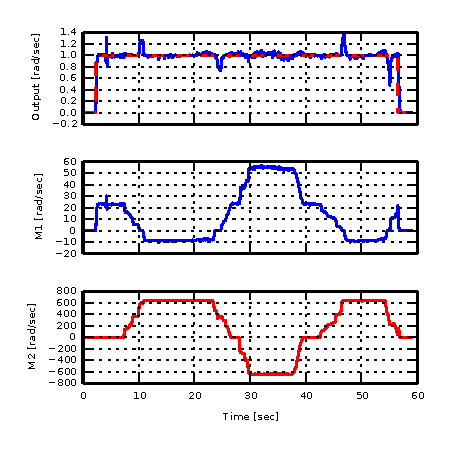
\includegraphics[width=0.75\textwidth]{dsdm_nullspace.pdf}
	\caption[DSDM actuator tracking constant output velocity: nullspace]{DSDM actuator tracking constant output velocity while sending manual command in the nullspace }
	\label{fig:dsdm_nullspace}
\end{figure}


\subsection{Seamless Transitions}

\subsubsection{Constant Speed}

Fig. \ref{fig:dsdm_cstspd_shifts} illustrates the DSDM actuator maintaining a constant output speed while shifting back-and-forth between high-speed and high-force mode.

\begin{figure}[htp]
	\centering
		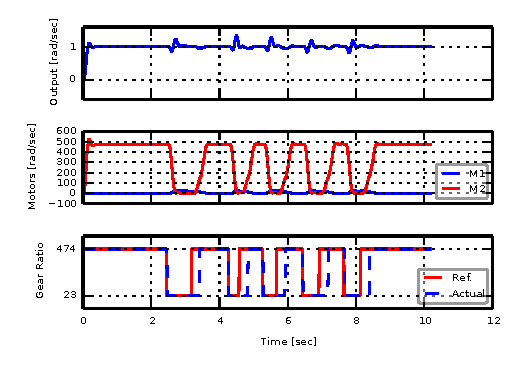
\includegraphics[width=0.75\textwidth]{dsdm_cstspd_shifts.pdf}
	\caption[DSDM actuator tracking constant output velocity: shifts]{DSDM actuator tracking constant output velocity while shifting back and forth between high-speed mode and high-force mode }
	\label{fig:dsdm_cstspd_shifts}
\end{figure}

Fig. \ref{fig:dsdm_cstspd_shifts_withprep} illustrates how the idea of preparation, by adjusting M2 velocity in the nullspace, improve the gear-shifting time. 

\begin{figure}[htp]
	\centering
		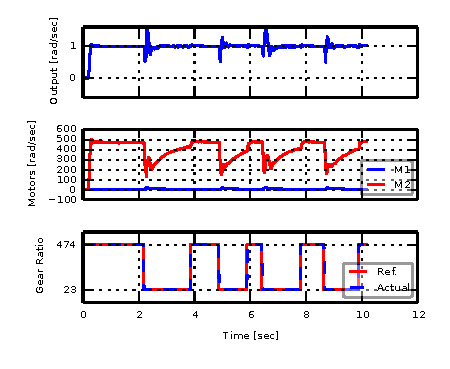
\includegraphics[width=0.75\textwidth]{dsdm_cstspd_shifts_withprep.pdf}
	\caption[DSDM actuator tracking constant output velocity: preparation]{DSDM actuator tracking constant output velocity while shifting back and forth between high-speed mode and high-force mode }
	\label{fig:dsdm_cstspd_shifts_withprep}
\end{figure}

Fig. \ref{fig:dsdm_cstspd_shifts_withprep_zoom} shows a zoom in on a fast down-shift with preparation. 

\begin{figure}[htp]
	\centering
		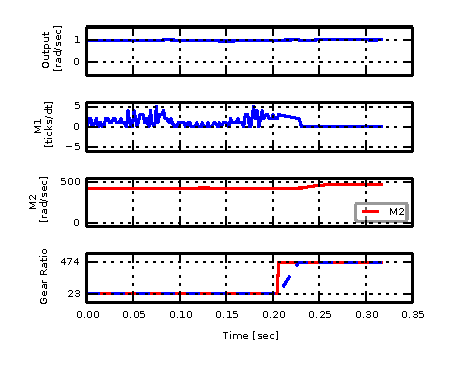
\includegraphics[width=0.75\textwidth]{dsdm_cstspd_shifts_withprep_zoom.pdf}
	\caption{ Fast down-shift }
	\label{fig:dsdm_cstspd_shifts_withprep_zoom}
\end{figure}

\subsubsection{Contact with a Compliant Load}

Experiment of the actuator making contact with a spring-like compliant load are illustrated at Fig. \ref{fig:dsdm_compliant_HF} using high-force mode, at Fig. \ref{fig:dsdm_compliant_HS} using high-speed mode and at \ref{fig:dsdm_ballon_down_shift_nice2} using both mode: making a down-shift as soon as contact is detected. 

\begin{figure}[htp]
	\centering
		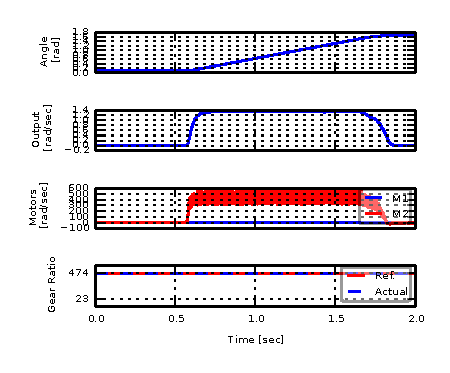
\includegraphics[width=0.75\textwidth]{dsdm_compliant_HF.pdf}
	\caption{ Contact with a compliant load in high-force mode }
	\label{fig:dsdm_compliant_HF}
\end{figure}

\begin{figure}[htp]
	\centering
		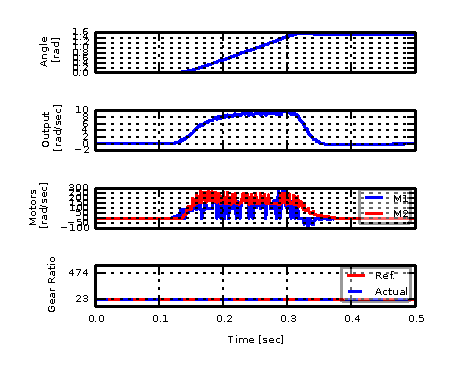
\includegraphics[width=0.75\textwidth]{dsdm_compliant_HS.pdf}
	\caption{ Contact with a compliant load in high-speed mode }
	\label{fig:dsdm_compliant_HS}
\end{figure}

%\begin{figure}[H]
	%\centering
		%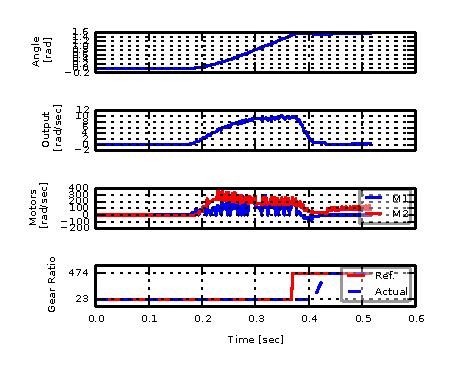
\includegraphics[width=0.95\textwidth]{dsdm_compliant_down.pdf}
	%\caption{ Fast downshift during a contact with a compliant load }
	%\label{fig:dsdm_compliant_down}
%\end{figure}
%
%\begin{figure}[H]
	%\centering
		%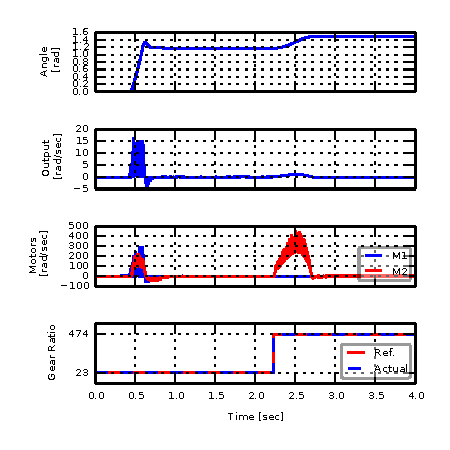
\includegraphics[width=0.95\textwidth]{dsdm_ballon_static.pdf}
	%\caption{ Fast downshift during a contact with a compliant load }
	%\label{fig:dsdm_ballon_static}
%\end{figure}
%
%\begin{figure}[H]
	%\centering
		%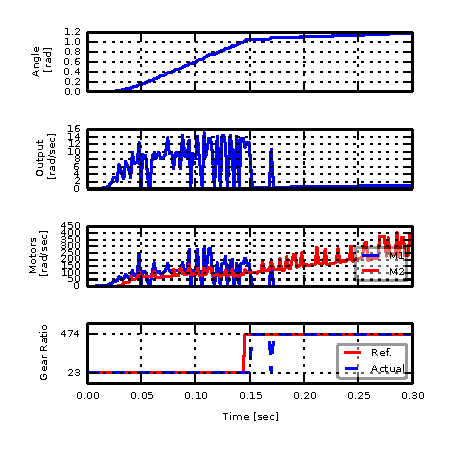
\includegraphics[width=0.95\textwidth]{dsdm_ballon_down_shift_nice.pdf}
	%\caption{ Fast downshift during a contact with a compliant load }
	%\label{fig:dsdm_ballon_down_shift_nice}
%\end{figure}

\begin{figure}[htp]
	\centering
		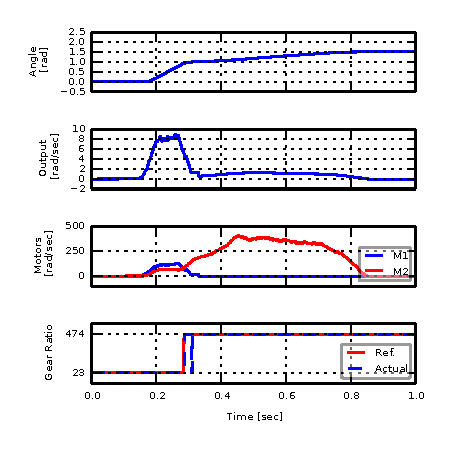
\includegraphics[width=0.75\textwidth]{dsdm_ballon_down_shift_nice2.pdf}
	\caption{ Fast downshift during a contact with a compliant load }
	\label{fig:dsdm_ballon_down_shift_nice2}
\end{figure}



\subsubsection{Impact with a Stiff Load}

Fig. \ref{fig:dsdm_stiff_down} illustrates an experiment where the DSDM make a quick down-shift after impacting a stiff heavy object. 

\begin{figure}[htp]
	\centering
		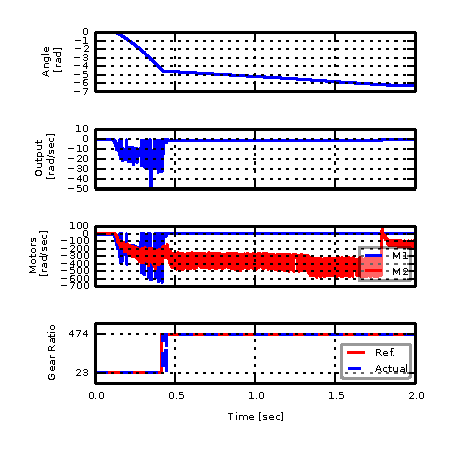
\includegraphics[width=0.75\textwidth]{dsdm_stiff_down.pdf}
	\caption{ Fast downshift during a contact with a heavy stiff load }
	\label{fig:dsdm_stiff_down}
\end{figure}

%
%\begin{figure}[htp]
	%\centering
		%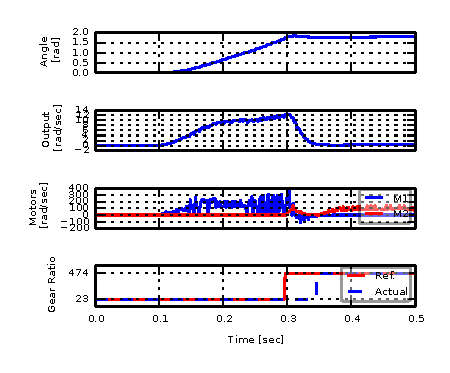
\includegraphics[width=0.75\textwidth]{dsdm_stiff_auto_new.pdf}
	%\caption{ Fast downshift during a contact with a fixed stiff load }
	%\label{fig:dsdm_stiff_auto_new}
%\end{figure}
%
%
%\begin{figure}[htp]
	%\centering
		%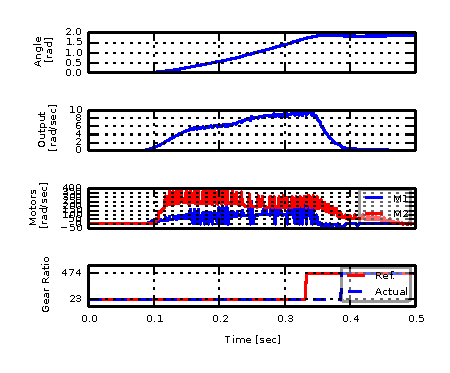
\includegraphics[width=0.75\textwidth]{dsdm_stiff_auto_nullspace_wrong.pdf}
	%\caption{ Fast downshift during a contact with a fixed stiff load }
	%\label{fig:dsdm_stiff_auto_nullspace_wrong}
%\end{figure}
